\chapter{Resultados}
\label{chap6}


Este capítulo apresenta e discute os resultados obtidos a partir da aplicação da metodologia proposta para a modelagem do sistema de destilação por membranas V-AGMD. Inicialmente, são realizadas análises exploratórias dos dados experimentais, com o objetivo de identificar relações entre as variáveis operacionais e as variáveis de saída do processo. Em seguida, avalia-se o desempenho do modelo físico reduzido (0D), utilizado como referência fenomenológica.

Posteriormente, são apresentados os resultados dos modelos orientados por dados, incluindo a comparação entre diferentes famílias de modelos e a análise de desempenho em termos de capacidade preditiva e generalização. Também são discutidos os critérios de seleção do modelo final, com base em validação cruzada, controle de complexidade.

Por fim, realiza-se a comparação entre o modelo físico reduzido e o modelo final selecionado, evidenciando os ganhos obtidos com a incorporação de abordagens híbridas físico--dados.

\section{Análise exploratória das relações entre variáveis de entrada e saídas experimentais}

Com o objetivo de investigar, de forma preliminar, possíveis associações entre as variáveis operacionais e as grandezas de interesse do processo V-AGMD, foram construídos gráficos de dispersão das variáveis de saída em função de cada variável de entrada. Essa análise tem caráter estritamente exploratório e busca identificar tendências visuais gerais nos dados experimentais, sem assumir, nesta etapa, qualquer forma funcional específica entre as variáveis.

Foram analisadas as variáveis de saída \(T_{\mathrm{out,alim}}\) (\textit{Alim\_T\_out}), \(T_{\mathrm{out,ref}}\) (\textit{Ref\_T\_out}) e o fluxo de permeado \(J\) (\textit{Flux}) em função das variáveis de entrada: temperatura de entrada da alimentação \(T_{\mathrm{in,alim}}\) (\textit{Alim\_T\_in}), temperatura de entrada da corrente de resfriamento \(T_{\mathrm{in,ref}}\) (\textit{Ref\_T\_in}), vazão da corrente de resfriamento \(\dot{V}_{\mathrm{ref}}\) (\textit{Ref\_V\_in}), pressão manométrica na câmara de ar \(P_{\mathrm{vac}}\) (\textit{P\_vacuum}) e concentração de NaCl \(C_{\mathrm{NaCl}}\) (\textit{C\_NaCl}).

De forma geral, observa-se que os dados experimentais se distribuem em faixas bem definidas ao longo dos eixos das variáveis de entrada, refletindo o planejamento experimental realizado em níveis operacionais discretos. Além disso, como as condições experimentais variam simultaneamente, os gráficos de dispersão devem ser interpretados com cautela, uma vez que as tendências observadas correspondem apenas a relações visuais univariadas e não isolam os efeitos combinados entre os diferentes parâmetros operacionais. Nesse sentido, a análise apresentada nesta seção não permite estabelecer relações causais nem quantificar a influência individual de cada variável, mas apenas destacar comportamentos visuais que podem orientar etapas posteriores da modelagem.

Para a saída \(T_{\mathrm{out,alim}}\), observa-se uma tendência visual de aumento mais evidente com a temperatura de entrada da corrente de resfriamento, conforme indicado no painel (b). Tendências diretas mais discretas também podem ser observadas em relação à temperatura de entrada da alimentação, à vazão da corrente de resfriamento e à pressão manométrica na câmara de ar, apresentadas nos painéis (a), (c) e (d), respectivamente. Já em relação à concentração de NaCl, painel (e), os dados apresentam maior dispersão, dificultando a identificação de uma tendência visual simples.

Para a saída \(T_{\mathrm{out,ref}}\), a tendência visual mais clara ocorre em função da temperatura de entrada da alimentação, como mostrado no painel (f). Esse comportamento é coerente com a troca térmica entre as correntes do sistema, uma vez que alterações na temperatura da alimentação tendem a se refletir na temperatura de saída da corrente de resfriamento. Nos demais painéis associados a essa saída, isto é, painéis (g), (h), (i) e (j), os dados aparecem mais dispersos ou organizados em faixas operacionais, sem indicar uma tendência visual univariada tão evidente.

No caso do fluxo de permeado \(J\), os painéis (k) e (m) sugerem tendências visuais de aumento associadas, respectivamente, à temperatura de entrada da alimentação e à vazão da corrente de resfriamento. Para a pressão manométrica na câmara de ar, painel (n), observa-se uma diferenciação entre as faixas de operação de vácuo, embora a dispersão dos dados impeça uma interpretação direta e isolada desse efeito. Em relação à concentração de NaCl, painel (o), nota-se uma tendência visual de redução do fluxo em condições de maior salinidade, ainda que com elevada variabilidade entre os pontos experimentais.

Dessa forma, a análise visual dos gráficos de dispersão sugere a presença de algumas tendências qualitativas entre entradas e saídas do sistema V-AGMD, mas também evidencia a limitação de interpretações baseadas em relações univariadas simples. A elevada dispersão dos dados e a combinação simultânea das condições operacionais reforçam a necessidade de modelos multivariados para representar de forma mais adequada o comportamento do processo.

A Figura~\ref{fig:scatter_vagmd} apresenta os gráficos de dispersão discutidos, organizando as três variáveis de saída em função das cinco variáveis de entrada avaliadas.

\begin{figure}[H]
    \centering
    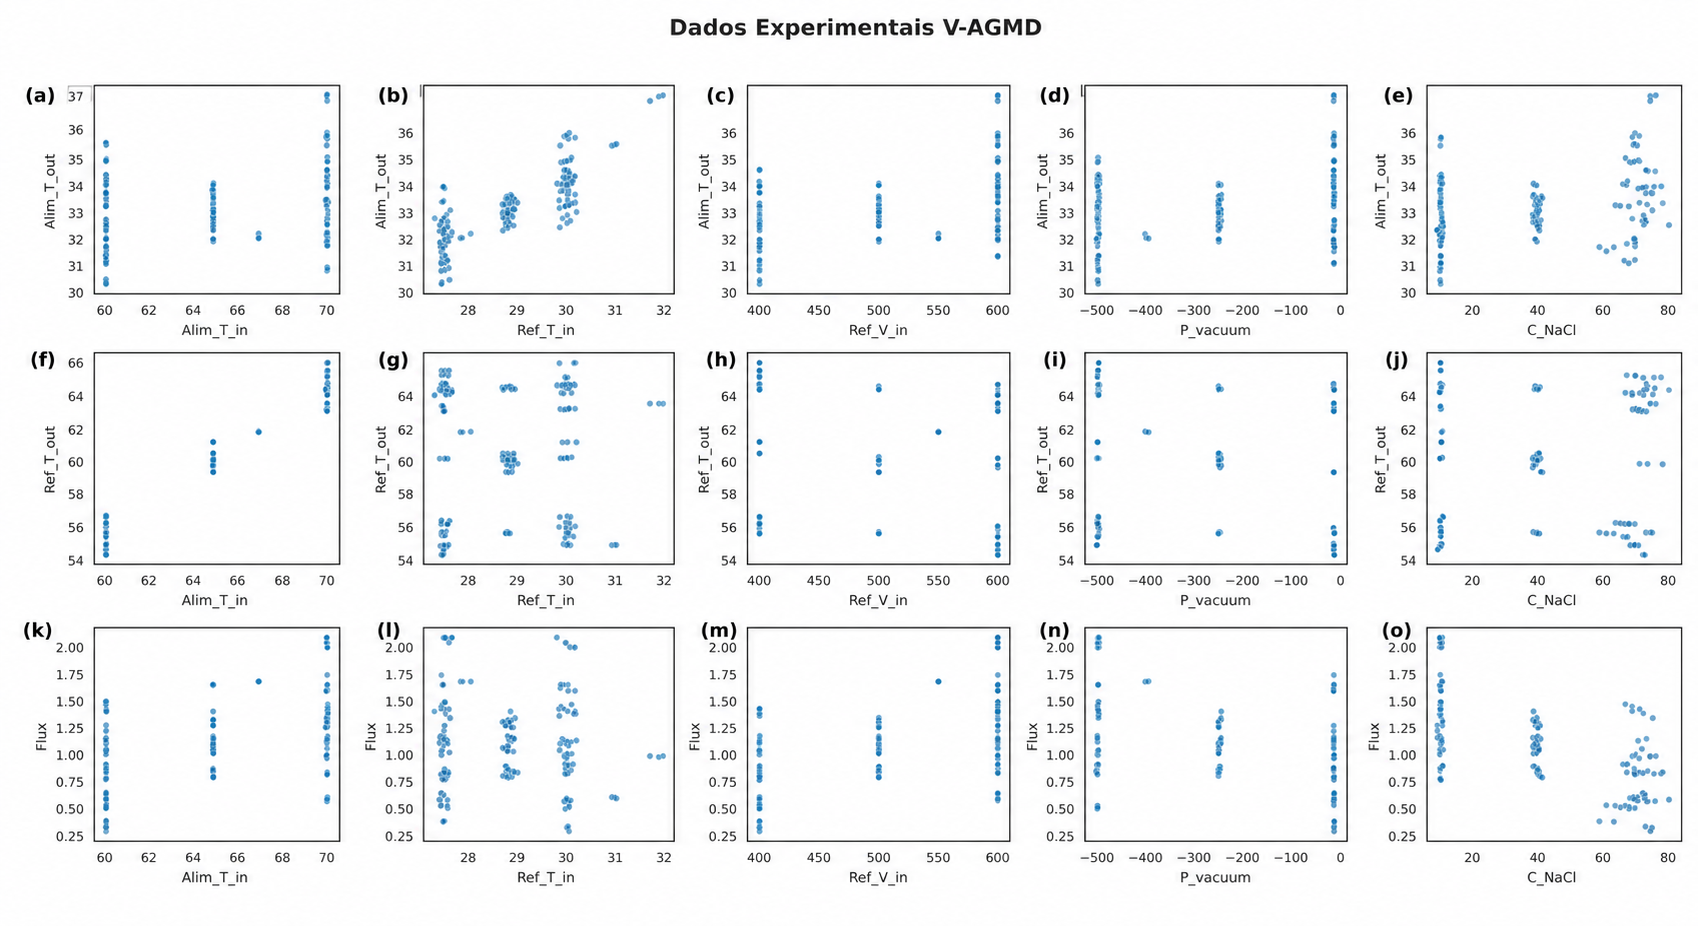
\includegraphics[angle=90, width=0.85\linewidth]{Imagens/chap06/scatter_vagmd_exp_only.png}
    \caption[Dispersão entre variáveis de entrada e saída do sistema V-AGMD]{Gráficos de dispersão entre as variáveis de entrada e as variáveis de saída experimentais do sistema V-AGMD. Fonte: Elaborado pela autora.}
    \label{fig:scatter_vagmd}
\end{figure}
\section{Análise de correlação entre variáveis de entrada e saída}
\label{subsec:correlacao_features_targets}

Com o objetivo de complementar a análise visual preliminar dos dados crus, foram calculados os coeficientes de correlação de Pearson e de Spearman entre as variáveis de entrada e as variáveis de saída do sistema. Conforme discutido na Fundamentação Teórica, esses coeficientes permitem avaliar diferentes formas de associação estatística entre variáveis, sem que isso implique uma relação causal direta entre elas.

Nesta etapa, a análise foi utilizada apenas como ferramenta exploratória, buscando identificar quais variáveis operacionais apresentam maior associação com cada resposta do sistema. A comparação entre os coeficientes de Pearson e Spearman também permite verificar se as associações observadas são mais compatíveis com uma tendência aproximadamente linear ou com uma tendência monotônica mais geral. Assim, os resultados obtidos servem como apoio à interpretação inicial dos dados e à discussão posterior do desempenho dos modelos preditivos.

A Figura~\ref{fig:heatmap_pearson_features_targets} apresenta o mapa de correlação dos coeficientes de correlação de Pearson entre as variáveis de entrada e os alvos. Observa-se que as temperaturas de saída, $Alim\_T_{out}$ e $Ref\_T_{out}$, exibem correlações lineares fortes com variáveis térmicas específicas. No caso das variáveis térmicas, observa-se que as maiores correlações ocorrem entre temperaturas de entrada e saída associadas às correntes que participam diretamente da troca de calor no módulo. Em particular, \(T_{\mathrm{out,alim}}\) (\textit{Alim\_T\_out}) apresenta correlação positiva elevada com a temperatura de entrada da corrente de arrefecimento, \(T_{\mathrm{in,ref}}\) (\textit{Ref\_T\_in}), indicando que o nível térmico da corrente fria influencia a temperatura final da alimentação após a passagem pelo módulo. De forma análoga, \(T_{\mathrm{out,ref}}\) (\textit{Ref\_T\_out}) apresenta correlação positiva elevada com a temperatura de entrada da alimentação, \(T_{\mathrm{in,alim}}\) (\textit{Alim\_T\_in}). Esse comportamento é coerente com a transferência de calor interna ao módulo, na qual parte da energia térmica da corrente de alimentação é transferida para a corrente de arrefecimento, tanto por condução através das camadas do sistema quanto pelo calor associado ao vapor d'água que permeia e condensa. Consequentemente, temperaturas mais elevadas da alimentação tendem a contribuir para maiores temperaturas de saída da corrente de arrefecimento.

\begin{figure}[H]
    \centering
    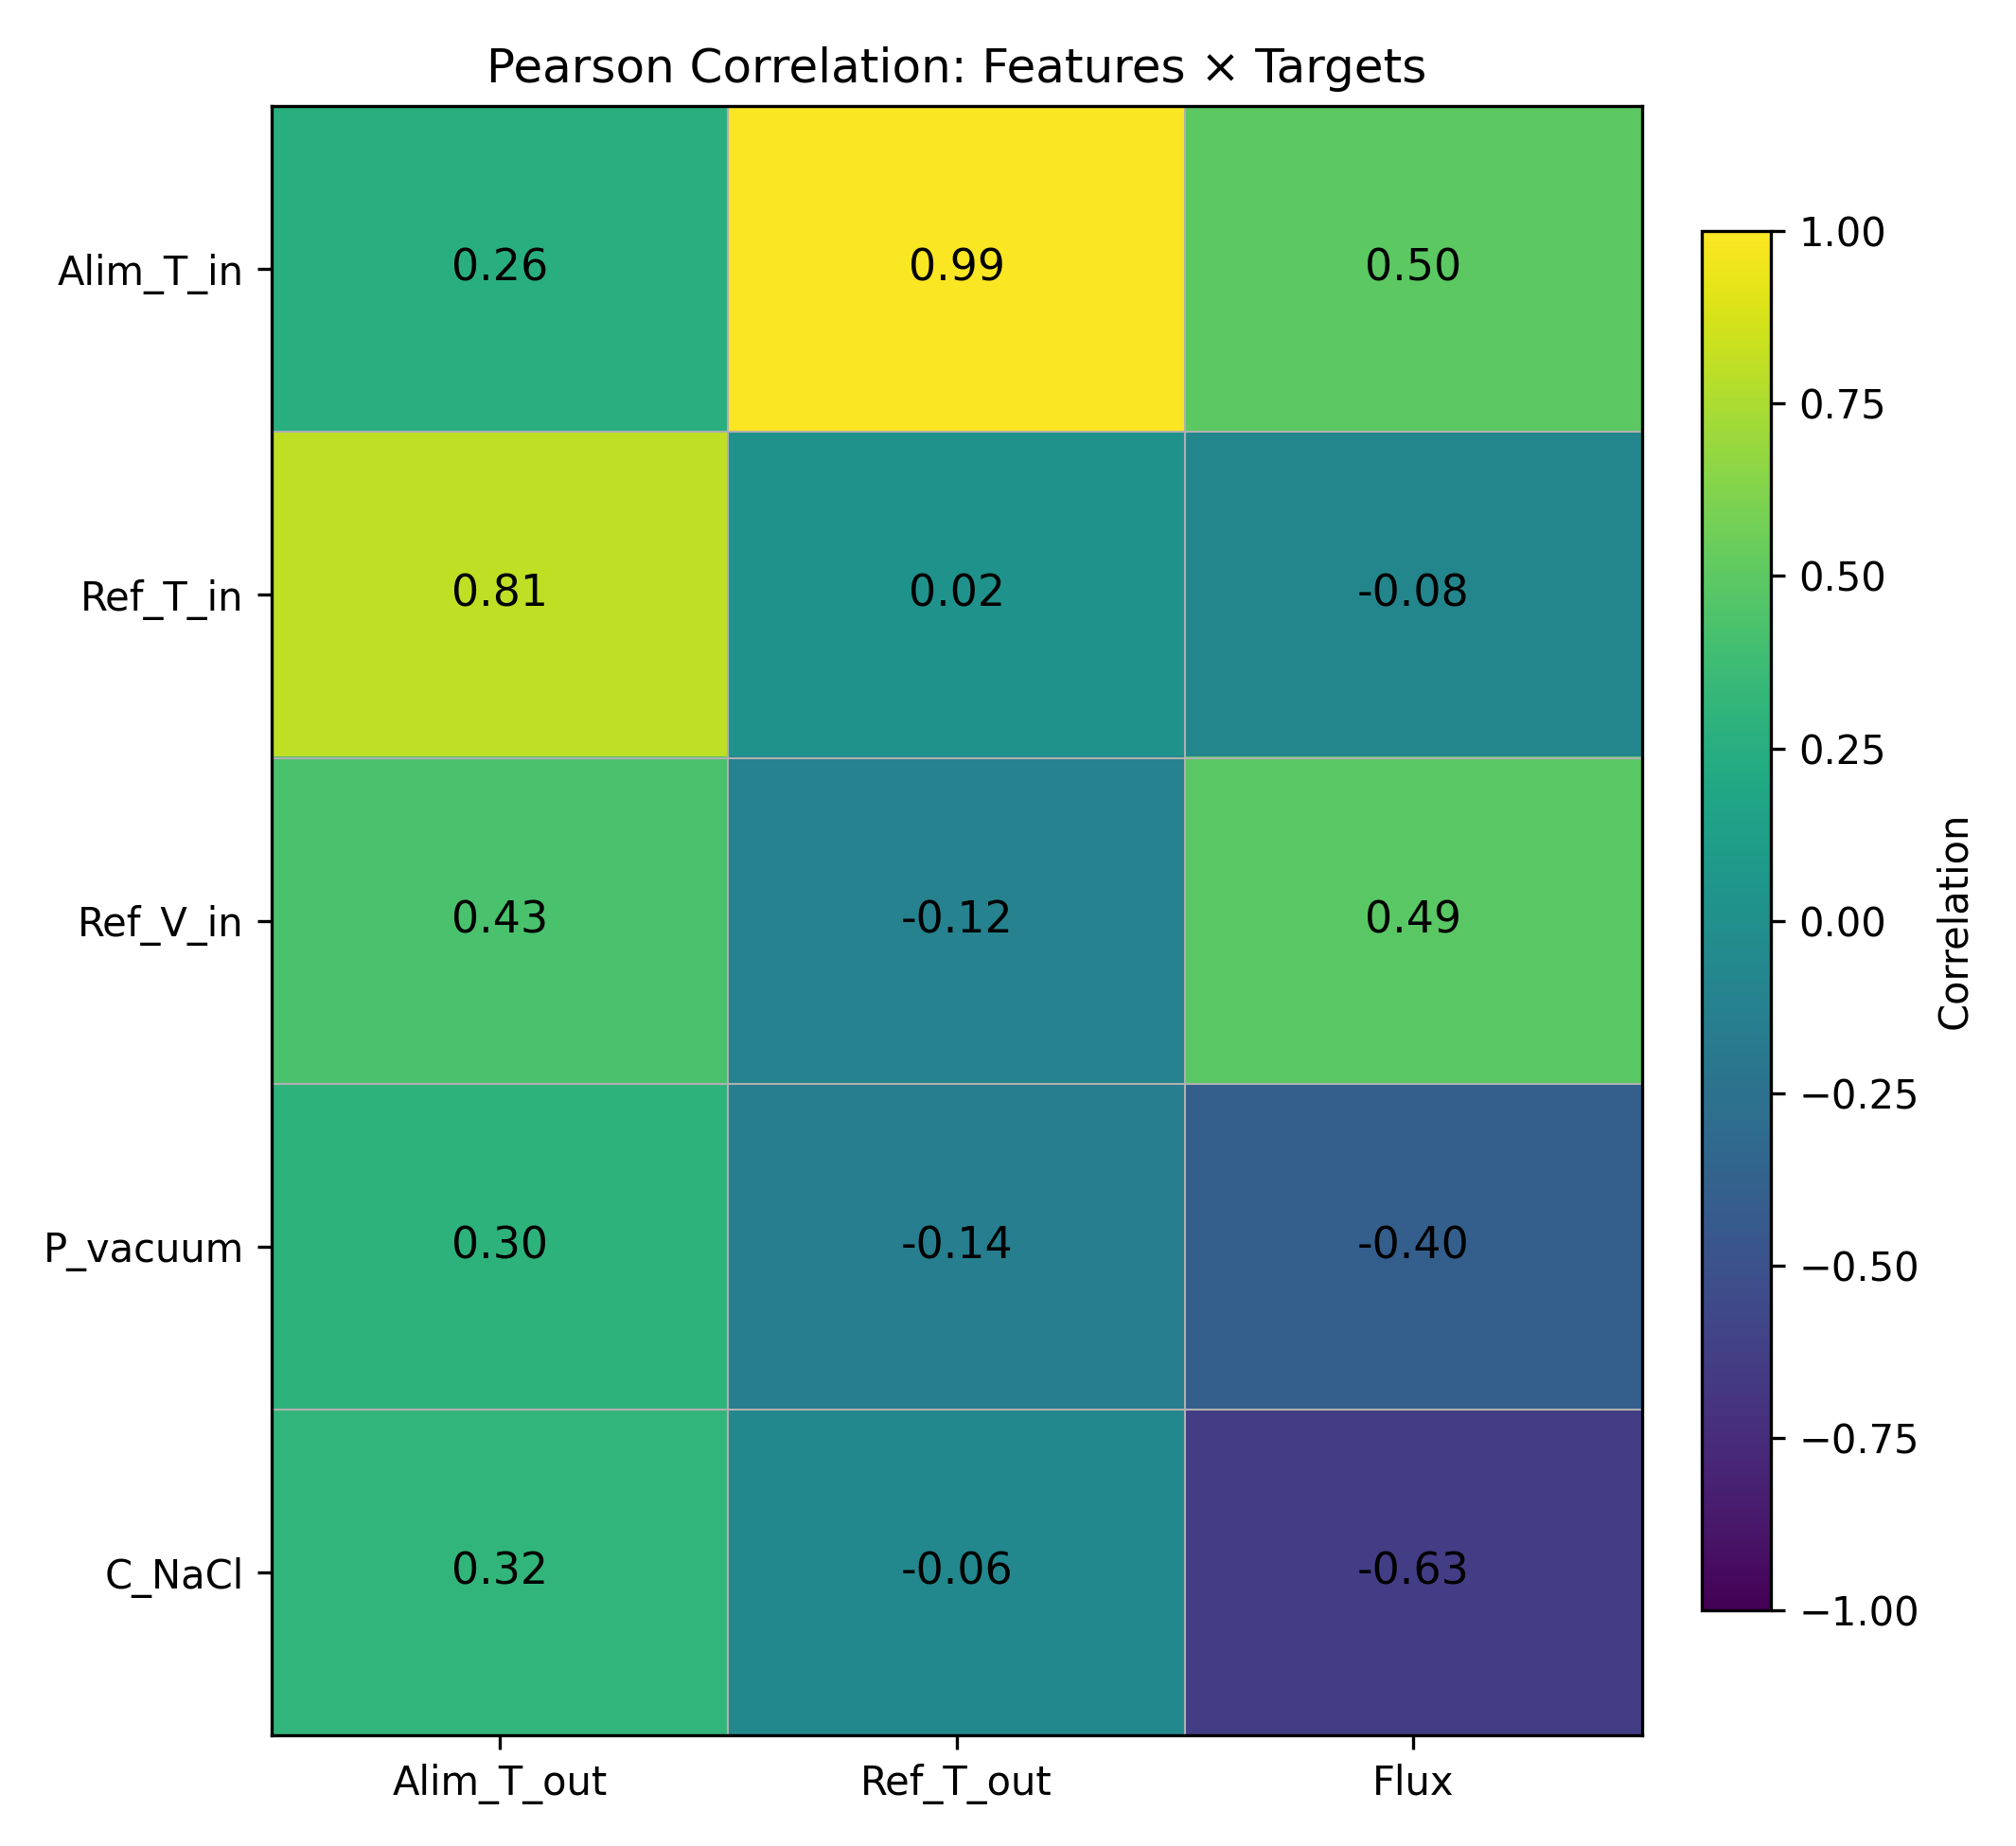
\includegraphics[width=0.9\textwidth]{Imagens/chap06/heatmap_pearson_features_targets.png}
    \caption[Correlação de Pearson entre variáveis do sistema]{Mapa de calor dos coeficientes de correlação de Pearson entre as variáveis de entrada e as variáveis de saída do sistema, utilizado para identificar possíveis relações lineares entre os parâmetros operacionais e as variáveis de desempenho do processo. Fonte: Autor.}
    \label{fig:heatmap_pearson_features_targets}
\end{figure}

Para o fluxo de permeado ($Flux$), a análise de Pearson indica apenas correlações lineares moderadas com variáveis individuais, destacando-se a correlação negativa com a concentração de sal ($C_{NaCl}$) e com a pressão de vácuo ($P_{vac}$), bem como correlações positivas moderadas com a temperatura de alimentação ($Alim\_T_{in}$) e a vazão da solução salina ($\dot{V}_{ref}$). A ausência de correlações lineares fortes sugere que o comportamento do fluxo não é dominado por uma única variável de entrada quando analisado de forma isolada.

A Figura~5.3 apresenta o mapa de correlação correspondente aos coeficientes de correlação de Spearman. De modo geral, observa-se que, para as temperaturas de saída, os valores de Spearman são próximos aos de Pearson, indicando que as relações dominantes são não apenas monotônicas, mas também aproximadamente lineares no domínio experimental considerado. Esse resultado é coerente com a interpretação física discutida anteriormente, segundo a qual as temperaturas de saída são fortemente influenciadas pela troca de calor entre a corrente de alimentação e a corrente de arrefecimento no interior do módulo. Em particular, o aumento da temperatura de entrada de uma corrente tende a afetar a temperatura de saída da outra, devido à transferência de energia térmica por condução através das camadas do sistema e pelo calor associado ao vapor d'água que permeia e condensa.

Os gráficos de dispersão foram mantidos como etapa qualitativa preliminar por evidenciarem a estrutura discreta do planejamento experimental e a sobreposição de efeitos entre variáveis operacionais. No entanto, a interpretação quantitativa das associações foi conduzida principalmente a partir dos mapas de correlação.

\begin{figure}[H]
    \centering
    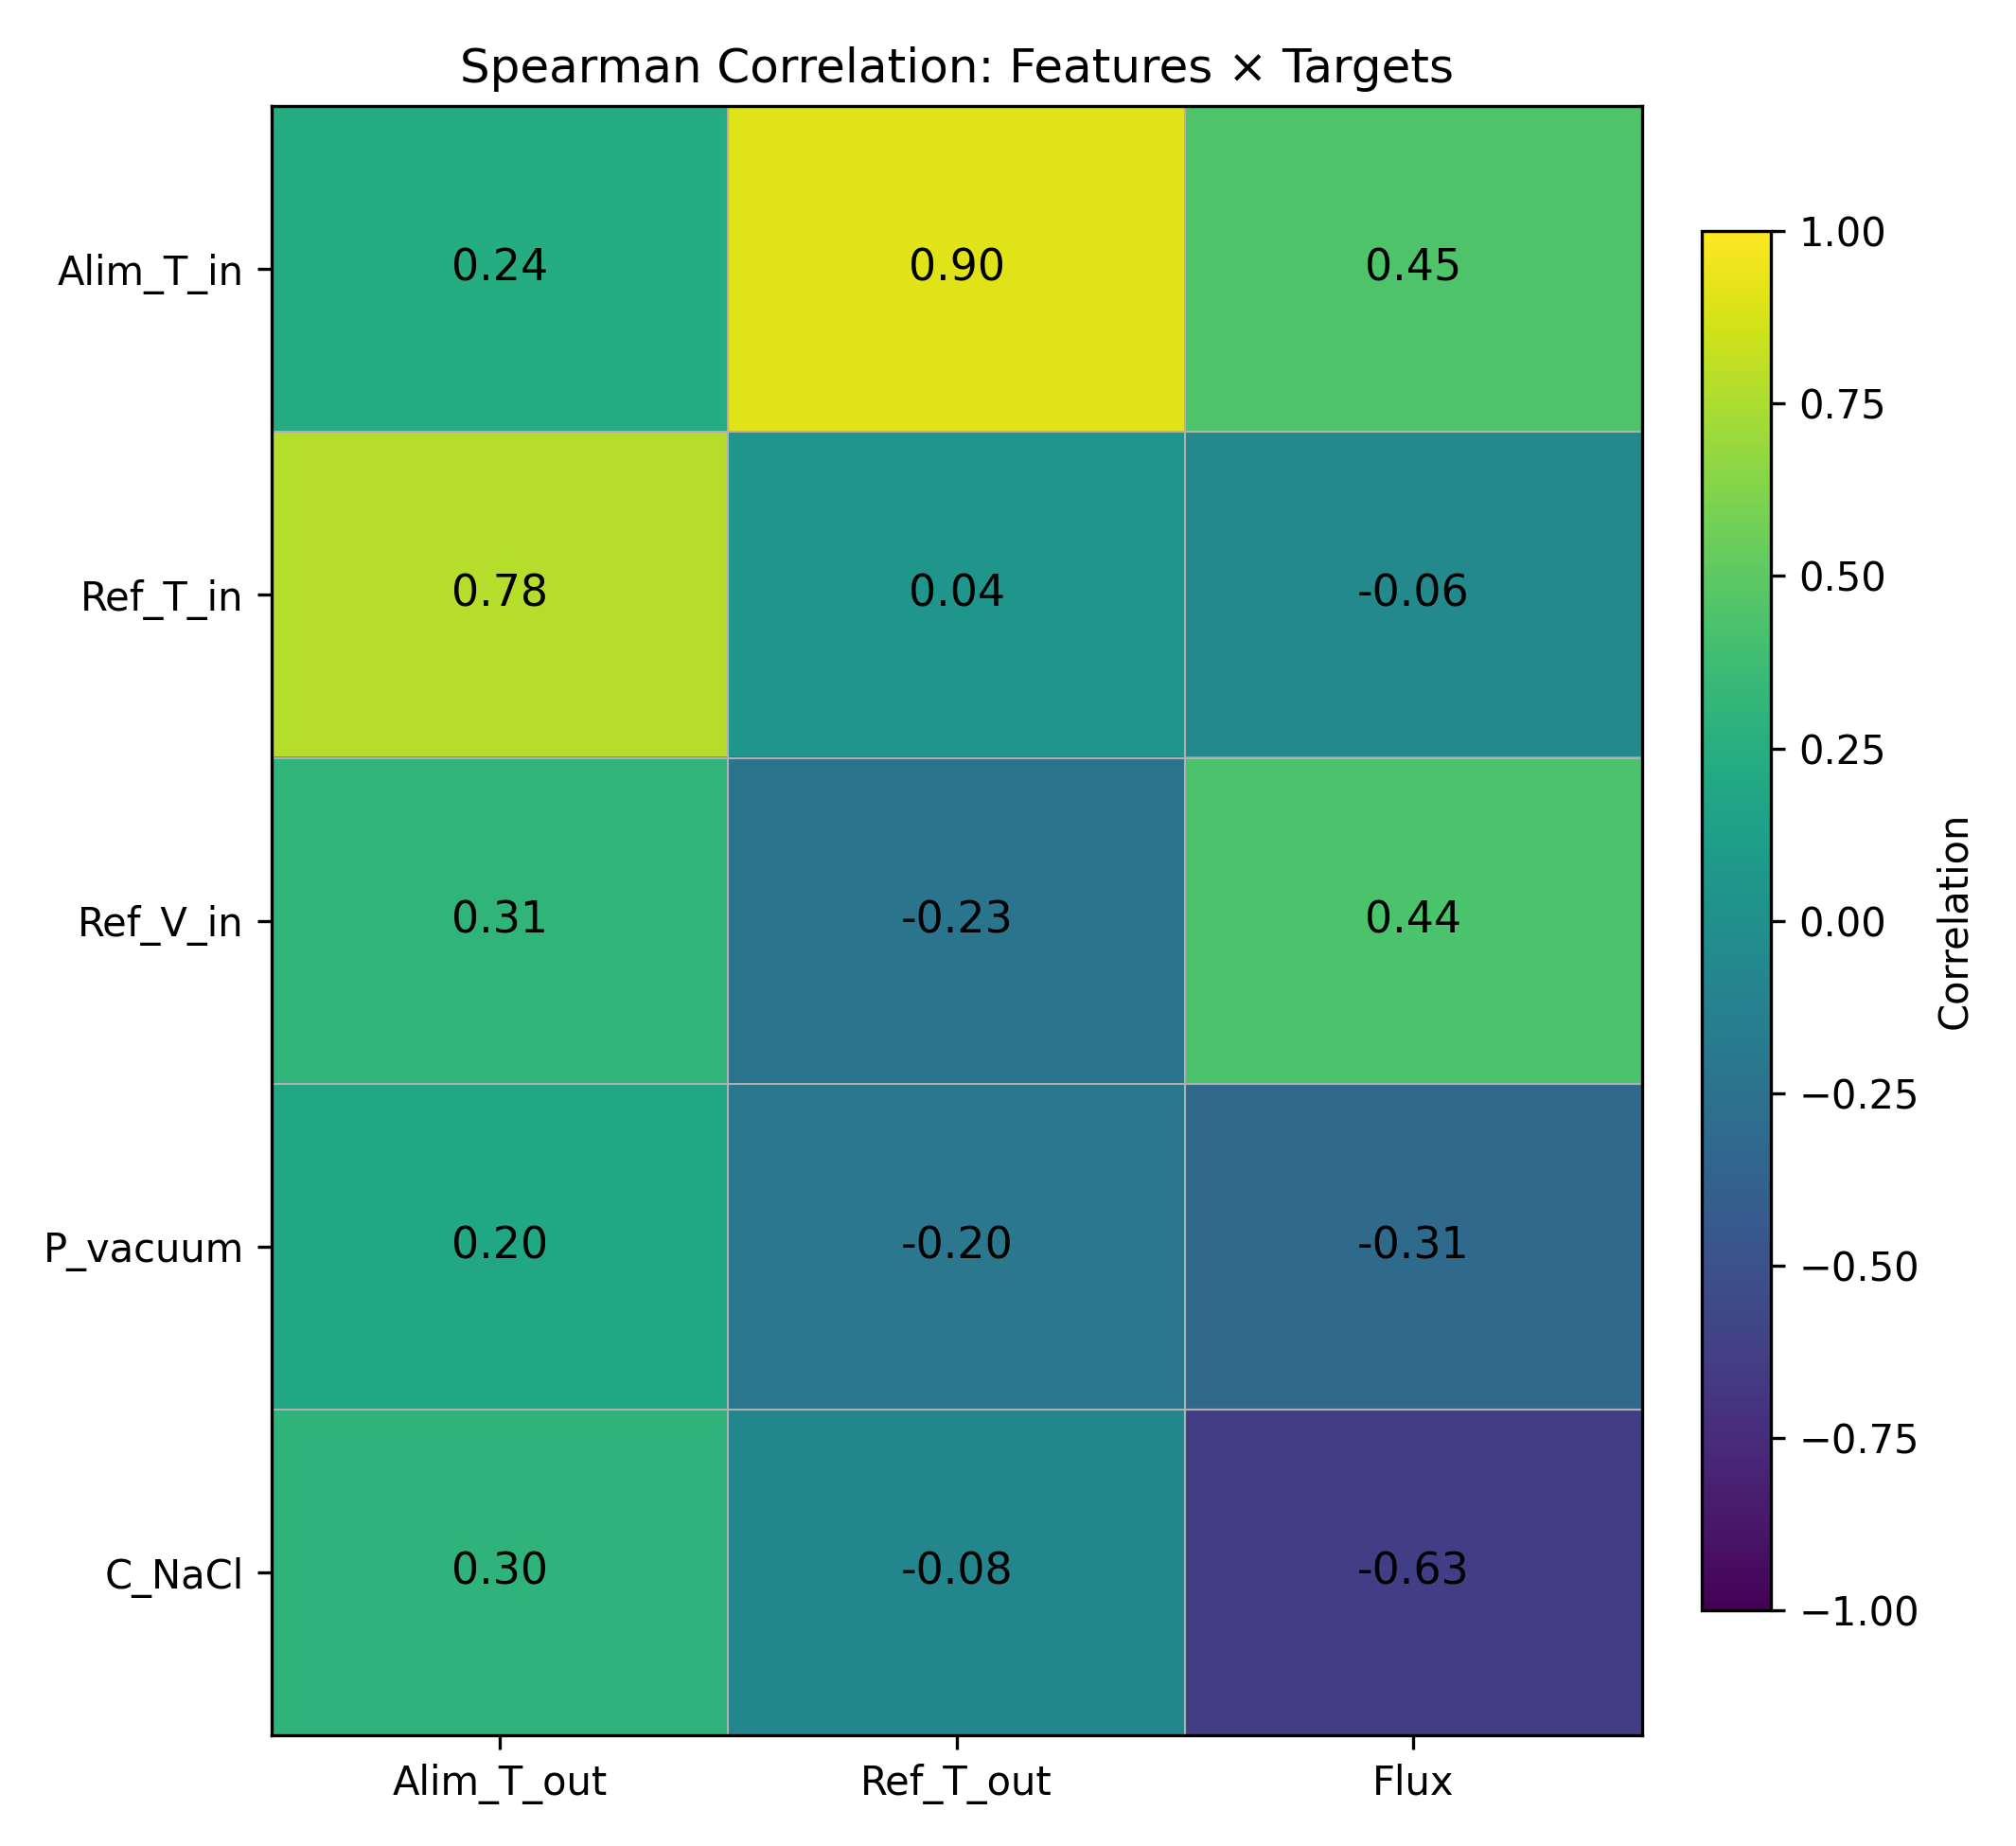
\includegraphics[width=0.9\textwidth]{Imagens/chap06/heatmap_spearman_features_targets.png}
    \caption[Correlação de Spearman entre variáveis do sistema]{Mapa de calor dos coeficientes de correlação de Spearman entre as variáveis de entrada e as variáveis de saída do sistema, utilizado para identificar relações monotônicas entre os parâmetros operacionais e as variáveis de desempenho do processo. Fonte: Autor.}
    \label{fig:heatmap_spearman_features_targets}
\end{figure}

No caso do fluxo de permeado, a proximidade entre os coeficientes de Pearson e de Spearman indica que as relações entre o fluxo e as variáveis operacionais são predominantemente monotônicas, porém distribuídas entre múltiplas variáveis, sem evidência de não linearidades marginais pronunciadas quando cada entrada é considerada isoladamente. Esse comportamento sugere que a complexidade do fluxo decorre principalmente de interações multivariadas entre condições operacionais, o que limita a interpretação baseada exclusivamente em correlações univariadas.

Em conjunto, os mapas de correlação reforçam as conclusões da análise visual preliminar: as temperaturas de saída apresentam comportamento fortemente governado por relações lineares dominantes, enquanto o fluxo de permeado não pode ser adequadamente descrito por relações lineares simples com variáveis individuais. Esses resultados motivam análises adicionais baseadas em gráficos de dispersão condicionais e em métodos de validação cruzada, capazes de capturar efeitos de interação e avaliar o impacto dessas relações no desempenho preditivo dos modelos.

\section{Avaliação do desempenho do modelo físico reduzido (0D)}
\label{subsec:avaliacao_modelo_0d}

Antes da aplicação dos modelos orientados por dados, avaliou-se o comportamento do modelo físico reduzido (0D) utilizado como referência fenomenológica neste trabalho. O objetivo desta análise não foi recalibrar ou propor modificações ao modelo físico, mas verificar como suas estimativas se comportam quando aplicadas às condições experimentais disponíveis e em que medida elas reproduzem as variáveis de saída de interesse.

O modelo 0D foi executado a partir das variáveis operacionais medidas experimentalmente: temperatura de entrada da alimentação \(T_{\mathrm{in,alim}}\), temperatura de entrada da corrente de arrefecimento \(T_{\mathrm{in,ref}}\), vazão volumétrica da solução salina \(\dot{V}_{\mathrm{in}}\), pressão manométrica na câmara de ar \(P_{\mathrm{man}}\) e concentração de NaCl \(C_{\mathrm{NaCl}}\). As saídas calculadas pelo modelo físico foram então comparadas com os valores experimentais correspondentes de temperatura de saída da alimentação, temperatura de saída da corrente de arrefecimento e fluxo de permeado.

Inicialmente, realizou-se uma verificação preliminar utilizando os dados experimentais reportados no trabalho em que o modelo físico reduzido foi originalmente proposto (\cite{Lisboa2024}). Essa etapa teve como finalidade apenas verificar a consistência da aplicação local do código em C disponibilizado, incluindo a leitura das variáveis de entrada, as conversões de unidades necessárias e a extração das saídas calculadas. Portanto, essa verificação não corresponde a uma nova validação do modelo físico, mas a uma etapa de controle antes de sua aplicação ao conjunto de dados experimental utilizado neste trabalho.

A Figura~\ref{fig:flux_article_vs_exp} apresenta a comparação entre o fluxo de permeado experimental e o fluxo de permeado calculado pelo modelo 0D. Em \ref{fig:flux_article_vs_exp}(a), são utilizados os dados experimentais reportados na literatura; em \ref{fig:flux_article_vs_exp}(b), são utilizados os dados experimentais deste trabalho. Em ambos os casos, a linha diagonal representa a concordância ideal entre o valor experimental e o valor calculado pelo modelo.

\begin{figure}[H]
    \centering
    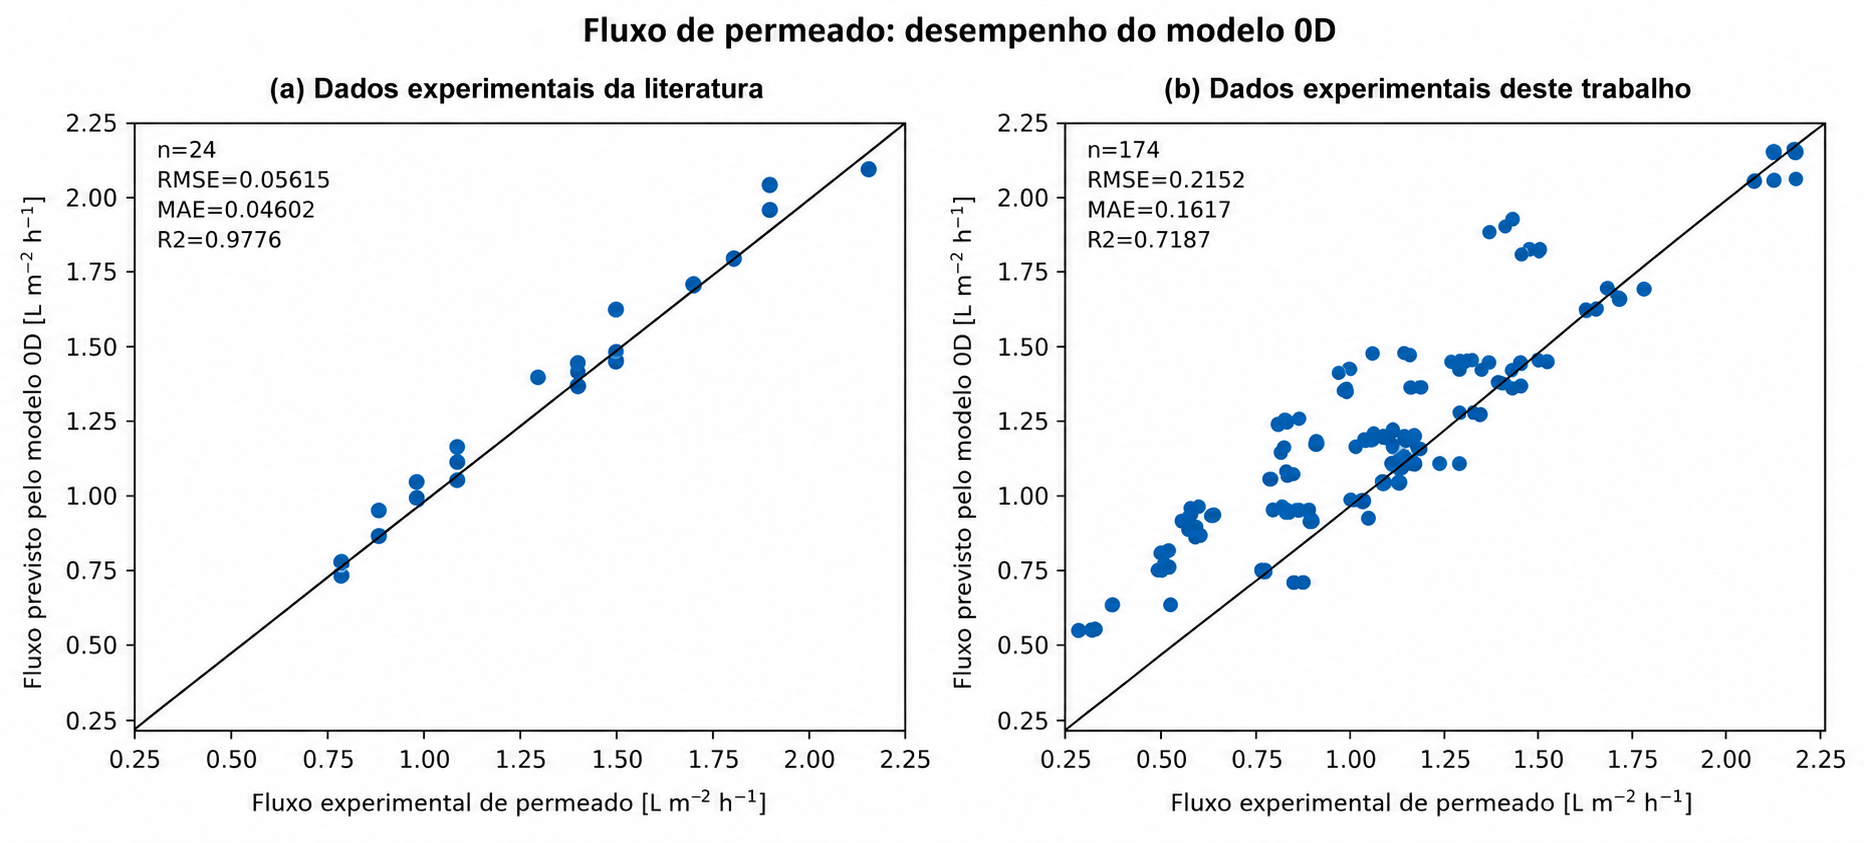
\includegraphics[width=0.9\linewidth]{Imagens/chap06/compare_flux_0d.png}
    \caption[Desempenho do modelo físico 0D na predição do fluxo de permeado]{Comparação entre o fluxo de permeado experimental e o fluxo de permeado calculado pelo modelo físico reduzido (0D). Em (a), são apresentados os dados experimentais reportados na literatura; em (b), são apresentados os dados experimentais deste trabalho. A linha diagonal indica a concordância ideal entre valores experimentais e calculados pelo modelo.}
    \fonte{Elaborado pela autora.}
    \label{fig:flux_article_vs_exp}
\end{figure}

% Após a atualização da figura, acrescentar na legenda:
% As barras de erro representam a incerteza associada às medidas experimentais de fluxo.

Observa-se que, para os dados experimentais da literatura, os pontos se distribuem próximos à reta de concordância, indicando que a execução local do modelo reproduz de forma consistente o comportamento reportado para o conjunto de dados usado como referência. Esse resultado é importante porque confirma que o procedimento computacional adotado neste trabalho está coerente com a formulação original do modelo físico.

Quando o modelo é aplicado aos dados experimentais deste trabalho, entretanto, observa-se maior dispersão em relação à reta identidade. Esse comportamento indica que o modelo 0D ainda acompanha a tendência global do fluxo de permeado, mas não reproduz integralmente a variabilidade observada no novo conjunto experimental. Essa diferença pode estar associada tanto às condições operacionais específicas avaliadas neste trabalho quanto às simplificações inerentes à formulação reduzida do modelo, que representa o módulo de forma concentrada e não descreve explicitamente variações espaciais ao longo dos canais.

Além da comparação para o fluxo de permeado, também foram avaliadas as demais variáveis de saída consideradas no problema de regressão. As Figuras~\ref{fig:alim_t_out_0d}, \ref{fig:ref_t_out_0d} e \ref{fig:flux_0d_exp} apresentam, respectivamente, as comparações entre valores experimentais e valores calculados pelo modelo 0D para a temperatura de saída da alimentação, a temperatura de saída da corrente de arrefecimento e o fluxo de permeado.

\begin{figure}[H]
    \centering
    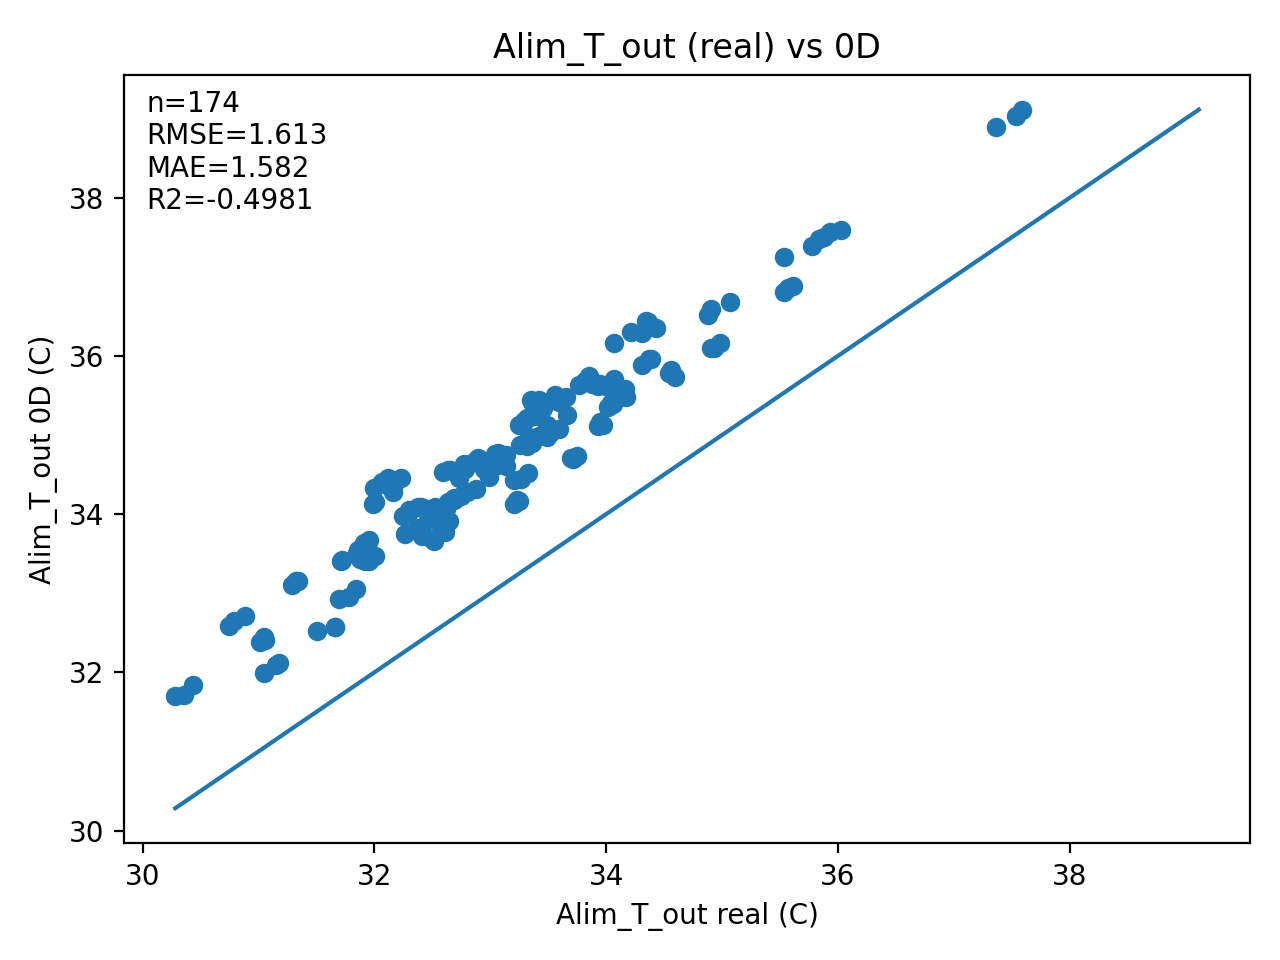
\includegraphics[width=0.7\linewidth]{Imagens/chap06/alim_T_out_real_vs_0d.png}
    \caption[Predição da temperatura de saída da alimentação pelo modelo 0D]{Comparação entre a temperatura de saída da alimentação medida experimentalmente e a temperatura calculada pelo modelo físico reduzido (0D). A linha diagonal indica a concordância ideal entre valores experimentais e calculados pelo modelo.}
    \fonte{Elaborado pela autora.}
    \label{fig:alim_t_out_0d}
\end{figure}

\begin{figure}[H]
    \centering
    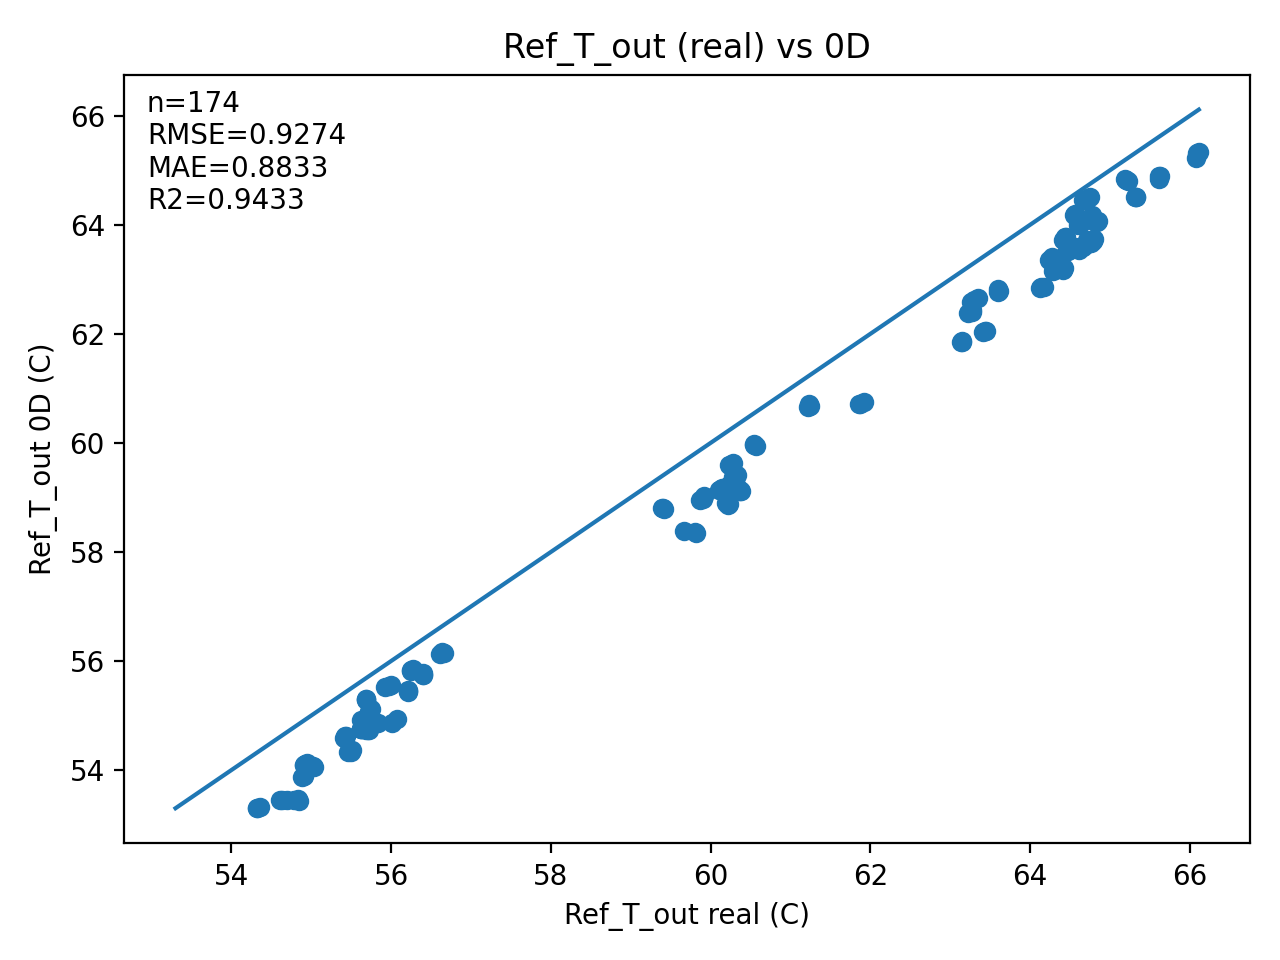
\includegraphics[width=0.7\linewidth]{Imagens/chap06/ref_T_out_real_vs_0d.png}
    \caption[Predição da temperatura de saída da corrente de arrefecimento pelo modelo 0D]{Comparação entre a temperatura de saída da corrente de arrefecimento medida experimentalmente e a temperatura calculada pelo modelo físico reduzido (0D). A linha diagonal indica a concordância ideal entre valores experimentais e calculados pelo modelo.}
    \fonte{Elaborado pela autora.}
    \label{fig:ref_t_out_0d}
\end{figure}

\begin{figure}[H]
    \centering
    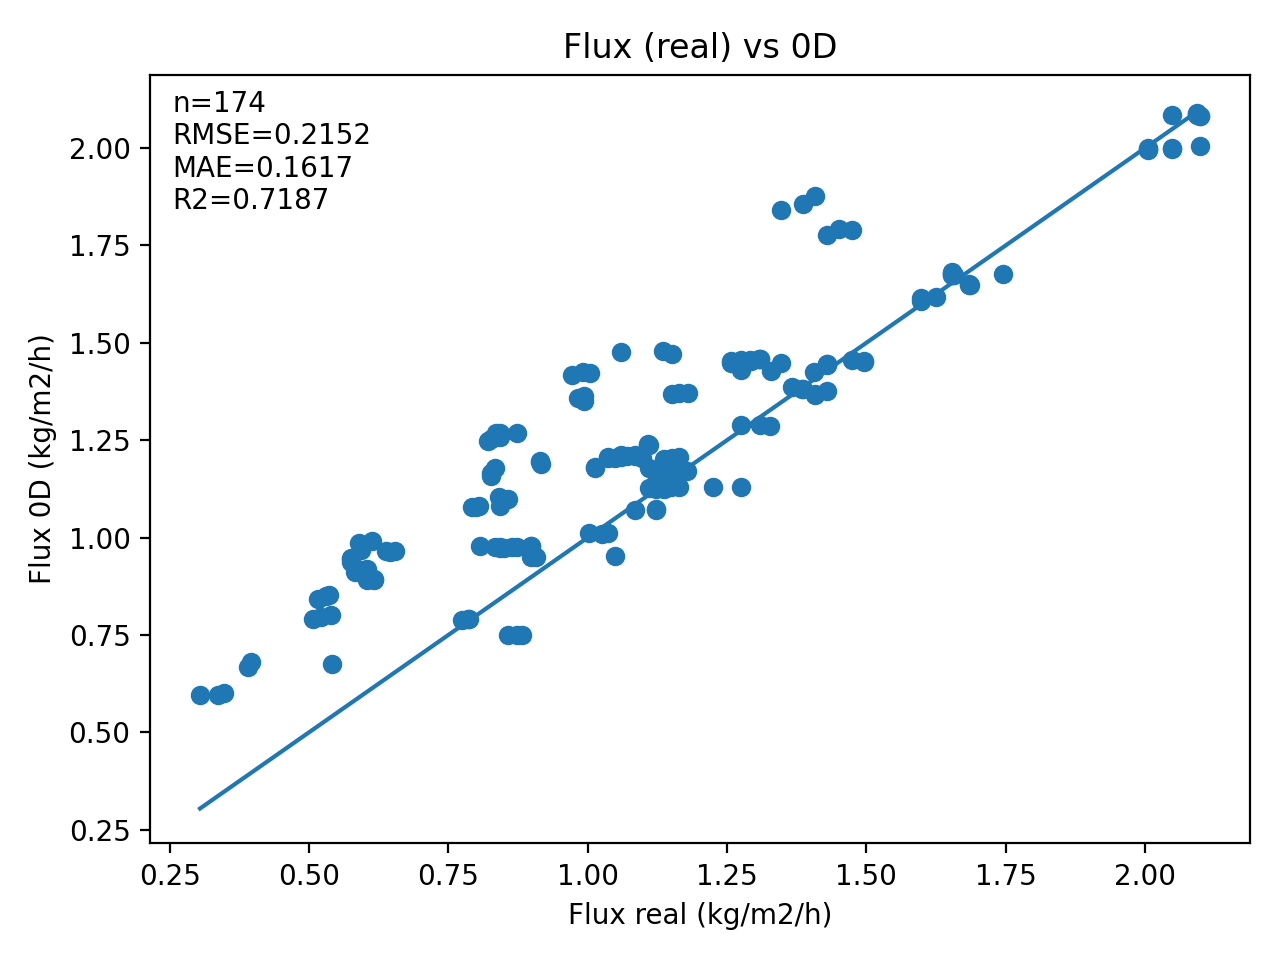
\includegraphics[width=0.7\linewidth]{Imagens/chap06/flux_real_vs_0d.png}
    \caption[Predição do fluxo de permeado pelo modelo 0D]{Comparação entre o fluxo de permeado medido experimentalmente e o fluxo calculado pelo modelo físico reduzido (0D). A linha diagonal indica a concordância ideal entre valores experimentais e calculados pelo modelo.}
    \fonte{Elaborado pela autora.}
    \label{fig:flux_0d_exp}
\end{figure}

A análise conjunta dessas três variáveis mostra que o desempenho do modelo 0D não é uniforme para todas as saídas. A melhor aderência ocorre para \(T_{\mathrm{out,ref}}\), sugerindo que o modelo representa de forma mais adequada a resposta térmica da corrente de arrefecimento. Esse resultado é coerente com a estrutura do modelo físico, que descreve diretamente os balanços de energia associados à transferência de calor entre as correntes no interior do módulo.

Para o fluxo de permeado, o comportamento é intermediário. O modelo acompanha a tendência geral dos dados, mas apresenta dispersão mais elevada em relação à reta de concordância. Isso indica que a formulação reduzida captura parte dos efeitos físicos dominantes associados à transferência de massa, mas não descreve completamente a variabilidade experimental do fluxo. Essa limitação é esperada, uma vez que o fluxo depende de fenômenos acoplados de transferência de calor e massa, incluindo diferenças locais de temperatura, pressão parcial de vapor, salinidade e condições de escoamento.

Já para \(T_{\mathrm{out,alim}}\), observa-se maior viés sistemático, indicando que o modelo tende a se afastar de forma mais consistente dos valores experimentais. Esse comportamento sugere que a temperatura de saída da alimentação é mais sensível a efeitos não capturados integralmente pela formulação 0D, como variações espaciais de temperatura ao longo do canal, perdas térmicas, heterogeneidades no escoamento ou simplificações nas resistências térmicas adotadas.

Portanto, a avaliação do modelo 0D cumpre dois papéis nesta etapa do trabalho. Primeiro, ela mostra que o modelo físico constitui uma referência fenomenológica relevante, capaz de representar tendências gerais do sistema e de fornecer estimativas fisicamente interpretáveis. Segundo, evidencia que essas estimativas não reproduzem integralmente os dados experimentais deste trabalho, especialmente para o fluxo de permeado e para a temperatura de saída da alimentação. Essa constatação justifica a investigação posterior de modelos orientados por dados e de estratégias híbridas físico--dados, nas quais as previsões do modelo 0D são utilizadas como informação auxiliar, mas combinadas à capacidade de ajuste dos métodos de aprendizado de máquina.
\section{Avaliação comparativa dos pipelines baseados em dados}
\label{subsec:avaliacao_pipelines_dados}

Após a avaliação do modelo físico reduzido, investigou-se o desempenho de modelos orientados por dados para a predição simultânea das três variáveis de saída consideradas neste trabalho: temperatura de saída da alimentação ($Alim\_T_{out}$), temperatura de saída do circuito de referência ($Ref\_T_{out}$) e fluxo de permeado ($Flux$). O objetivo dessa etapa não foi apenas comparar diferentes famílias de modelos, mas também estabelecer um \textit{pipeline} de modelagem compatível com as características do conjunto de dados experimental disponível.

Inicialmente, foram examinadas duas diferentes estratégias de pré-processamento, incluindo a utilização direta dos dados experimentais e a discretização de variáveis de entrada por meio de \textit{binning}. As análises preliminares indicaram, entretanto, que a abordagem de discretização não produziu ganhos consistentes de desempenho ou generalização no problema estudado. Dessa forma, a etapa completa de seleção e comparação entre modelos foi conduzida utilizando apenas o pipeline baseado nos dados experimentais originais.

\subsection{Estratégia de análise dos resultados}
\label{subsubsec:estrategia_validacao}

Os resultados apresentados nesta seção foram obtidos a partir do procedimento de validação cruzada agrupada por \textit{Regime} e do critério hierárquico de seleção descritos no Capítulo de Metodologia. Portanto, os detalhes do particionamento dos dados, da busca de hiperparâmetros e da regra de seleção não são retomados aqui. A presente seção concentra-se na interpretação comparativa do desempenho dos modelos selecionados em cada família.

A análise foi conduzida tomando o fluxo de permeado como variável prioritária de comparação, pois essa grandeza representa diretamente a produtividade do processo V-AGMD. Em outras palavras, a escolha das configurações foi orientada principalmente pela capacidade de prever a taxa de produção de permeado por área de membrana, que é o indicador mais diretamente associado ao desempenho operacional do sistema. As temperaturas de saída também foram avaliadas, mas como variáveis complementares para verificar se a priorização do fluxo comprometia a representação do comportamento térmico do módulo.

Dessa forma, a discussão dos resultados é organizada em três etapas. Primeiro, compara-se o desempenho global das famílias de modelos com base no RMSE do fluxo de permeado. Em seguida, avalia-se o comportamento dos modelos selecionados para as três variáveis de saída, permitindo verificar a qualidade preditiva de forma conjunta. Por fim, são analisados os gráficos de valores preditos em função dos valores experimentais, com o objetivo de identificar padrões de aderência, dispersão e possíveis vieses nas previsões.
\subsection{Comparação global entre modelos}

A comparação global entre modelos tem como objetivo avaliar, de forma integrada, o desempenho das diferentes abordagens testadas no \textit{pipeline} de modelagem. A escolha dos modelos não foi conduzida apenas por tentativa e erro, mas organizada de forma progressiva para comparar alternativas com diferentes níveis de complexidade, capacidade de representação não linear e incorporação de conhecimento físico.

Para isso, os modelos foram agrupados em três classes principais: modelos clássicos de regressão, redes neurais puramente orientadas por dados e estratégias híbridas físico--dados. A Tabela~\ref{tab:familias_modelos_avaliados} resume o papel de cada grupo no processo de comparação.

\begin{table}[H]
\centering
\caption{Síntese das famílias de modelos avaliadas no \textit{pipeline}.}
\label{tab:familias_modelos_avaliados}
\small
\begin{tabular}{p{0.20\textwidth}p{0.28\textwidth}p{0.27\textwidth}p{0.17\textwidth}}
\toprule
Família de modelos & Modelos avaliados & Papel na comparação & Característica principal \\
\midrule
Modelos lineares clássicos & OLS, Ridge, Lasso e ElasticNet, incluindo formulações multitarefa e independentes & Servem como referência de menor complexidade para verificar se relações mais simples já descrevem parte do comportamento observado & Baixa complexidade e maior interpretabilidade \\
\midrule
Modelos baseados em árvores & Árvore de decisão, floresta aleatória e \textit{Gradient Boosting} & Avaliam se partições não lineares do espaço de entrada melhoram a predição em relação aos modelos lineares & Maior flexibilidade, com possível sensibilidade aos dados de treinamento \\
\midrule
Redes neurais puramente orientadas por dados & MLP e rede neural de referência & Avaliam se uma arquitetura neural, sem incorporação explícita de informação física, é suficiente para capturar relações não lineares entre entradas e saídas & Capacidade de aproximação não linear \\
\midrule
Modelos híbridos físico--dados & ZohanResidual, ZohanHPD, Luc e FrozenBaseline & Avaliam se a incorporação de informação proveniente do modelo físico reduzido melhora a predição em relação às abordagens puramente orientadas por dados & Combinação entre tendência física e correção aprendida por dados \\
\bottomrule
\end{tabular}
\end{table}

Todos os modelos e configurações foram avaliados sob o mesmo procedimento de validação cruzada agrupada por \textit{Regime}, conforme descrito na Metodologia. Dessa forma, as diferenças observadas no desempenho não refletem apenas a capacidade de ajuste aos dados de treinamento, mas também a capacidade dos modelos de generalizar para regimes experimentais mantidos fora do treinamento em cada partição da validação cruzada.

A leitura dos resultados desta seção deve considerar três aspectos principais. Primeiro, como o fluxo de permeado foi definido como variável prioritária de seleção, o desempenho em $Flux$ é o critério central para escolha do modelo final. Segundo, como o problema é multi-saída, é necessário verificar se o bom desempenho no fluxo é acompanhado por resultados adequados nas temperaturas de saída, $T_{\mathrm{alim,out}}$ e $T_{\mathrm{ref,out}}$. Terceiro, a comparação entre famílias permite avaliar se o ganho obtido decorre apenas do aumento de flexibilidade do modelo ou se a incorporação de informação física trouxe benefício adicional.

Nesse sentido, a Tabela~\ref{tab:model_performance_outputs} consolida os valores de RMSE e $R^2$ para as três variáveis de saída. Os valores reportados correspondem às métricas calculadas a partir das predições \textit{out-of-fold} (OOF), conforme descrito na Seção~\ref{sec:avaliacao_oof}. Diferentemente do RMSE médio de validação cruzada utilizado durante a seleção de hiperparâmetros, as métricas OOF são obtidas a partir de modelos retreinados independentemente em cada partição, reduzindo o viés de otimismo associado ao processo de seleção (\cite{Cawley2010Overfitting}). A linha destacada corresponde ao modelo híbrido ZohanResidual, selecionado como modelo final.

\begin{table}[H]
\centering
\caption[Desempenho OOF consolidado dos modelos avaliados]{Desempenho consolidado dos modelos avaliados com base nas predições \textit{out-of-fold} (OOF), ordenados pelo RMSE do fluxo de permeado. As métricas OOF são calculadas sobre predições de modelos retreinados independentemente em cada partição da validação cruzada (\cite{Cawley2010Overfitting}). A linha destacada corresponde ao modelo final selecionado.}
\label{tab:model_performance_outputs}
\begin{tabular}{l c c c c c c}
\toprule
\multirow{2}{*}{Modelo} & \multicolumn{2}{c}{\textbf{$Alim\_T_{out}$}} & \multicolumn{2}{c}{\textbf{$Ref\_T_{out}$}} & \multicolumn{2}{c}{\textbf{$Flux$}} \\
\cmidrule(lr){2-3} \cmidrule(lr){4-5} \cmidrule(lr){6-7}
 & R$^2$ & RMSE & R$^2$ & RMSE & R$^2$ & RMSE \\
\midrule
\multicolumn{7}{c}{\textbf{Modelos clássicos}} \\
\midrule
MLP\_sklearn & 0.922 & 0.368 & 0.925 & 1.067 & 0.970 & 0.071 \\
OLS & 0.965 & 0.246 & 0.996 & 0.251 & 0.952 & 0.089 \\
Lasso & 0.965 & 0.245 & 0.996 & 0.251 & 0.951 & 0.090 \\
Ridge & 0.962 & 0.257 & 0.989 & 0.401 & 0.938 & 0.101 \\
\midrule
\multicolumn{7}{c}{\textbf{Modelos híbridos}} \\
\midrule
\rowcolor{orange!15}
ZohanResidual & 0.951 & 0.290 & 0.990 & 0.385 & \textbf{0.978} & \textbf{0.061} \\
HRNN & 0.972 & 0.221 & 0.991 & 0.377 & 0.963 & 0.078 \\
Luc & 0.931 & 0.347 & 0.985 & 0.482 & 0.954 & 0.087 \\
FrozenBaseline & 0.968 & 0.237 & 0.990 & 0.394 & 0.949 & 0.091 \\
\midrule
\multicolumn{7}{c}{\textbf{Modelo físico de referência}} \\
\midrule
Modelo físico 0D & -0.498 & 1.613 & 0.943 & 0.927 & 0.719 & 0.215 \\
\bottomrule
\end{tabular}
\end{table}

A partir da Tabela~\ref{tab:model_performance_outputs}, observa-se que o modelo híbrido ZohanResidual apresentou a melhor combinação global de desempenho. Para o alvo prioritário $Flux$, esse modelo obteve o menor RMSE (0,061) e o maior R² (0,978) entre as configurações avaliadas, representando uma redução de 33\% no RMSE em relação ao modelo puramente orientado por dados (FrozenBaseline, RMSE 0,091). Esse ganho evidencia que a incorporação da informação física, por meio da arquitetura residual, permitiu ao modelo aprender correções mais precisas para a predição do fluxo de permeado.

O modelo HRNN, que utiliza a arquitetura residual com concatenação total das entradas, também apresentou ganho significativo, com RMSE de 0,078 e R² de 0,963. O modelo Luc, que utiliza regularização física na função de perda, apresentou desempenho intermediário (RMSE 0,087), enquanto o FrozenBaseline, puramente orientado por dados, obteve RMSE de 0,091. Esses resultados indicam que a estratégia de incorporação da física influencia diretamente o ganho preditivo: a abordagem residual (ZohanResidual) mostrou-se mais eficaz do que a regularização na perda (Luc) para o problema em questão.

Para complementar a leitura da Tabela~\ref{tab:model_performance_outputs}, a Figura~\ref{fig:ranking_rmse_targets} apresenta o ranking dos modelos em função do RMSE para cada uma das três variáveis de saída. Diferentemente da figura anterior, que mostrava apenas o fluxo de permeado, esta visualização permite verificar se a ordenação dos modelos se mantém quando são consideradas também as temperaturas de saída. Os nomes dos modelos utilizados na figura são os mesmos adotados na tabela, de modo a facilitar a comparação direta entre as duas representações.

\begin{figure}[H]
\centering

\includegraphics[width=1\textwidth]{Imagens/chap06/rmse_by_target_grouped.png}
\caption[Ranking dos modelos por RMSE para cada variável de saída]{Ranking dos modelos avaliados com base no erro quadrático médio da raiz (RMSE) para cada variável de saída do sistema: fluxo de permeado, temperatura de saída da alimentação e temperatura de saída do circuito de resfriamento. Os nomes dos modelos seguem a mesma nomenclatura apresentada na Tabela~\ref{tab:model_performance_outputs}. Fonte: Autor.}
\label{fig:ranking_rmse_targets}
\end{figure}

A Figura~\ref{fig:ranking_rmse_targets} evidencia que o modelo ZohanResidual permanece entre os melhores modelos nos três alvos avaliados. No caso do $Flux$, sua posição no topo do ranking confirma sua adequação ao critério principal de seleção. Para as temperaturas de saída, o desempenho também se mantém competitivo, com menor RMSE em relação às demais abordagens avaliadas. Esse comportamento reforça que o modelo selecionado não apresentou bom desempenho apenas no alvo priorizado, mas também preservou qualidade preditiva nas demais respostas do sistema.

Dessa forma, os resultados indicam que o modelo mais indicado para o objetivo principal deste trabalho é o modelo híbrido ZohanResidual. Essa escolha não decorre apenas do uso de uma arquitetura mais complexa, mas do ganho preditivo observado para o fluxo de permeado, aliado à incorporação de informação física e à manutenção de desempenho satisfatório para as demais variáveis de saída. Os modelos lineares permanecem relevantes como referências de comparação, pois mostram que parte do comportamento do sistema pode ser descrita por relações mais simples. No entanto, para a finalidade central deste estudo, que é prever o desempenho do processo V-AGMD com foco no fluxo de permeado, a abordagem híbrida apresentou a melhor combinação entre erro, generalização e coerência física.
\subsection{Interpretação física do desempenho dos modelos}
\label{subsec:interpretacao_fisica_modelos}

A análise dos resultados obtidos mostra que o desempenho dos modelos não foi uniforme para todas as variáveis de saída. As temperaturas de saída da alimentação, $T_{\mathrm{alim,out}}$, e do circuito de resfriamento, $T_{\mathrm{ref,out}}$, apresentaram resultados satisfatórios para diferentes famílias de modelos. Já a predição do fluxo de permeado, $Flux$, mostrou maior sensibilidade à escolha da arquitetura de modelagem, sendo o alvo para o qual a abordagem híbrida apresentou ganho mais expressivo.

Esse comportamento deve ser interpretado considerando que, no processo de destilação por membranas, os fenômenos de transferência de calor e massa estão diretamente acoplados. O fluxo de permeado depende dos gradientes térmicos e da diferença de pressão de vapor estabelecida através da membrana, enquanto as temperaturas de saída também são consequência dos fenômenos de transporte que ocorrem no módulo. A evaporação e a condensação do permeado envolvem calor latente e modificam os balanços de energia nas correntes de alimentação e resfriamento, de modo que $T_{\mathrm{alim,out}}$ e $T_{\mathrm{ref,out}}$ não devem ser interpretadas como variáveis independentes do fluxo.

Assim, o fato de alguns modelos de menor complexidade terem apresentado desempenho satisfatório para as temperaturas de saída não significa que essas variáveis sejam fisicamente desacopladas ou necessariamente simples. Esse resultado indica apenas que, dentro da faixa operacional analisada e para o conjunto de dados disponível, parte da variação de $T_{\mathrm{alim,out}}$ e $T_{\mathrm{ref,out}}$ pôde ser representada adequadamente por diferentes abordagens de modelagem. Essa interpretação é específica para os dados avaliados neste trabalho e não deve ser generalizada para outras condições operacionais sem validação adicional.

No caso do fluxo de permeado, o melhor desempenho da arquitetura híbrida pode ser interpretado como consequência da natureza acoplada dessa variável. O fluxo não depende apenas de uma variável operacional isolada, mas resulta da combinação entre gradientes de temperatura, diferença de pressão de vapor através da membrana, resistências térmicas e difusivas e efeitos de polarização. Como a pressão de vapor apresenta dependência não linear com a temperatura, pequenas alterações nas condições térmicas e operacionais podem gerar variações não proporcionais no fluxo. Dessa forma, o $Flux$ concentra de maneira mais evidente os efeitos combinados de transferência de calor e massa presentes no processo V-AGMD.

Nesse contexto, o ganho obtido pelo modelo híbrido ZohanResidual na predição do fluxo sugere que essa arquitetura foi capaz de representar melhor essas interações. A informação proveniente do modelo físico reduzido fornece uma estimativa inicial baseada nos principais mecanismos fenomenológicos do sistema, enquanto a rede neural aprende correções associadas aos desvios observados nos dados experimentais. Portanto, o melhor resultado para o fluxo de permeado pode ser entendido como um indicativo de que a abordagem híbrida foi especialmente útil para capturar relações acopladas e não lineares entre as variáveis do processo.

Dessa forma, os modelos lineares não devem ser apresentados como alternativa preferencial, mas como referências de comparação. O fato de terem apresentado resultados satisfatórios em algumas variáveis indica apenas que parte do comportamento observado no intervalo experimental pode ser descrita por relações de menor complexidade. Entretanto, na comparação global, o modelo híbrido ZohanResidual apresentou a solução mais adequada aos objetivos do trabalho, por combinar menor erro para o alvo prioritário, $Flux$, com desempenho satisfatório para $T_{\mathrm{alim,out}}$ e $T_{\mathrm{ref,out}}$. Assim, a escolha do ZohanResidual se justifica não pela superioridade em uma variável isolada, mas pelo equilíbrio entre produtividade, representação térmica e capacidade de generalização.

Cabe destacar que o procedimento de seleção de modelos adotado priorizou explicitamente o erro associado ao fluxo de permeado, por este ser o principal indicador de produtividade do processo. As temperaturas de saída foram previstas simultaneamente no treinamento multi-saída, mas não foram utilizadas como critério principal na seleção de hiperparâmetros. Ainda assim, o modelo ZohanResidual manteve bom desempenho para $T_{\mathrm{alim,out}}$ e $T_{\mathrm{ref,out}}$, indicando que a arquitetura selecionada foi capaz de representar não apenas o alvo priorizado, mas também as respostas térmicas associadas ao funcionamento do sistema.

Dessa forma, o resultado obtido reforça a utilidade da abordagem híbrida proposta. A incorporação da informação proveniente do modelo físico reduzido fornece uma referência fenomenológica inicial, enquanto a rede neural aprende correções orientadas pelos dados experimentais. Essa combinação permitiu melhorar a predição do fluxo de permeado sem comprometer a qualidade das predições das temperaturas de saída, o que reforça a adequação do modelo ZohanResidual para o problema multi-saída analisado neste trabalho.
\section{Seleção do modelo final}
\label{subsec:analise_modelo_selecionado}

A etapa anterior permitiu identificar padrões consistentes de desempenho, robustez e complexidade entre as diferentes famílias de modelos avaliadas. Com base no critério hierárquico de seleção adotado neste trabalho, procedeu-se então à escolha formal da configuração final.

A arquitetura selecionada foi a \texttt{KerasMLP\_ZohanResidual\_Restricted}, por apresentar o melhor equilíbrio entre erro em validação cruzada e complexidade estrutural segundo a regra de seleção definida no Capítulo de Metodologia. O modelo obteve RMSE$_{Flux}$ em validação cruzada de aproximadamente 0,061 e RMSE OOF de 0,061, demonstrando alta estabilidade entre as duas estimativas.

Cabe destacar que as arquiteturas híbridas avaliadas neste trabalho não foram submetidas a uma nova busca ampla de hiperparâmetros. Inicialmente, realizou-se uma busca mais abrangente para definir a configuração da rede neural de referência, incluindo a escolha da arquitetura e de hiperparâmetros gerais de treinamento. Em seguida, essa configuração foi utilizada como base para a construção das estratégias híbridas.

Dessa forma, na etapa dedicada aos modelos híbridos, os hiperparâmetros gerais da rede foram mantidos fixos. A busca foi restrita apenas aos parâmetros específicos de cada estratégia híbrida, como o hiperparâmetro de regularização $L_2$ no caso da arquitetura ZohanResidual. Essa escolha reduziu o custo computacional do processo de seleção e permitiu avaliar o efeito da incorporação de informação física sem alterar simultaneamente toda a estrutura da rede neural.

\subsection{Critério de seleção baseado na regra 1-SE e complexidade do modelo}

Nesta subseção, apresenta-se o critério utilizado para selecionar as configurações de modelos ao longo do \textit{pipeline}. A seleção não ocorreu em uma única etapa, mas em momentos sucessivos: inicialmente, na definição da rede neural de referência e, posteriormente, no ajuste restrito da arquitetura híbrida ZohanResidual. Em ambos os casos, utilizou-se a regra \textit{1-standard error} (1-SE), combinada, quando aplicável, com um critério de controle da complexidade do modelo.

De forma geral, a regra 1-SE consiste em evitar a escolha automática da configuração com melhor desempenho médio em validação cruzada quando existem alternativas com desempenho semelhante dentro da variabilidade estimada. Como a métrica principal deste trabalho é o RMSE associado ao alvo $Flux$, valores menores de erro indicam melhor desempenho. No entanto, nos gráficos desta seção, o eixo vertical apresenta o escore usado no processo de seleção na convenção negativa associada ao RMSE. Portanto, valores mais próximos de zero correspondem a menores erros de predição.

Na primeira etapa, o critério foi aplicado durante a busca da rede neural de referência. Nessa fase, foram avaliadas diferentes configurações de arquitetura e hiperparâmetros, de modo que os modelos candidatos apresentavam diferentes níveis de complexidade estrutural. A Figura~\ref{fig:selection_plot_baseline} ilustra esse processo.
\subsection{Sensibilidade ao hiperparâmetro de regularização}

Antes da etapa de ajuste restrito da arquitetura híbrida, foi realizada uma busca inicial de hiperparâmetros para a rede neural de referência. Nessa etapa, além da definição da arquitetura da rede, analisou-se a sensibilidade do modelo ao hiperparâmetro de regularização $L_2$, responsável por penalizar a magnitude dos pesos e atuar como mecanismo de controle de sobreajuste.

Na Figura~\ref{fig:error_sweepparam_baseline}, observa-se que o menor erro médio de validação cruzada entre os valores avaliados ocorre em $\log_{10}(\lambda_{L2}) = -6$, que corresponde ao menor valor de regularização testado. Portanto, o gráfico não indica a presença de um mínimo interno para o hiperparâmetro analisado, mas sim que, dentro da faixa investigada, a rede neural de referência apresentou melhor desempenho em validação com uma penalização $L_2$ de baixa intensidade.

À medida que o valor de $\lambda_{L2}$ aumenta de $10^{-6}$ para $10^{-5}$ e $10^{-4}$, observa-se elevação do erro de validação, sugerindo que uma regularização mais intensa pode ter restringido excessivamente a flexibilidade da rede nessa etapa. Para $\lambda_{L2}=10^{-3}$, há uma redução parcial do erro em relação aos pontos anteriores, mas o valor permanece superior ao obtido com $\lambda_{L2}=10^{-6}$. Assim, a tendência observada não deve ser interpretada como monotônica, mas como uma indicação de que, para a faixa testada, o melhor compromisso entre ajuste e validação ocorreu no menor nível de regularização avaliado.

A presença simultânea dos erros de treinamento e validação também permite observar que o erro de treinamento permanece inferior ao erro de validação em todas as configurações, como esperado. A escolha do hiperparâmetro, contudo, foi guiada pelo desempenho estimado em validação cruzada, e não apenas pela capacidade de ajuste aos dados de treinamento. Dessa forma, a configuração selecionada busca preservar a capacidade preditiva do modelo em amostras não utilizadas no ajuste de cada dobra da validação cruzada.

\begin{figure}[H]
\centering

\includegraphics[width=0.82\textwidth]{Imagens/chap06/model_selection/agmd_stage1_baseline_dados_att_com_var_com_phy_error_vs_sweepparam_KerasMLP_BaselineSearch.png}
\caption[Variação do erro com a regularização $L_2$]{Variação do erro de predição em função do hiperparâmetro de regularização $L_2$ durante a etapa de ajuste da rede neural de referência. A linha tracejada indica o menor erro de validação cruzada observado entre os valores testados. A análise permite avaliar a influência da regularização no desempenho do modelo, evidenciando o compromisso entre ajuste aos dados de treinamento e capacidade de generalização. Fonte: Autor.}
\label{fig:error_sweepparam_baseline}
\end{figure}

Na Figura~\ref{fig:error_sweepparam_baseline}, observa-se que o menor erro médio de validação cruzada ocorre na região de $\log_{10}(\lambda_{L2}) = -6$. Esse comportamento indica que, para a rede neural de referência, a introdução de uma penalização $L_2$ de baixa magnitude foi suficiente para melhorar o desempenho em validação em relação às demais configurações avaliadas. Ao mesmo tempo, a presença simultânea dos erros de treinamento e validação permite observar que a escolha do hiperparâmetro não foi feita apenas pelo menor erro de treinamento, mas pelo desempenho estimado em dados não utilizados no ajuste de cada dobra da validação cruzada. Dessa forma, o valor selecionado representa um compromisso entre ajuste aos dados de treinamento e capacidade de generalização.

A arquitetura e os hiperparâmetros selecionados nessa etapa passaram a compor a configuração da rede neural de referência, utilizada como base para as estratégias híbridas avaliadas posteriormente no \textit{pipeline}. A partir dessa configuração inicial, a etapa de ajuste da arquitetura híbrida ZohanResidual manteve a estrutura da rede fixa, variando apenas o hiperparâmetro de regularização $L_2$. Essa escolha permitiu avaliar se, após a incorporação da informação proveniente do modelo físico reduzido, o desempenho do modelo continuava sensível à intensidade da regularização.

A Figura~\ref{fig:error_sweepparam_best_model} apresenta o comportamento do erro de validação cruzada ao longo dessa variação restrita para o modelo híbrido ZohanResidual.

\begin{figure}[H]
\centering
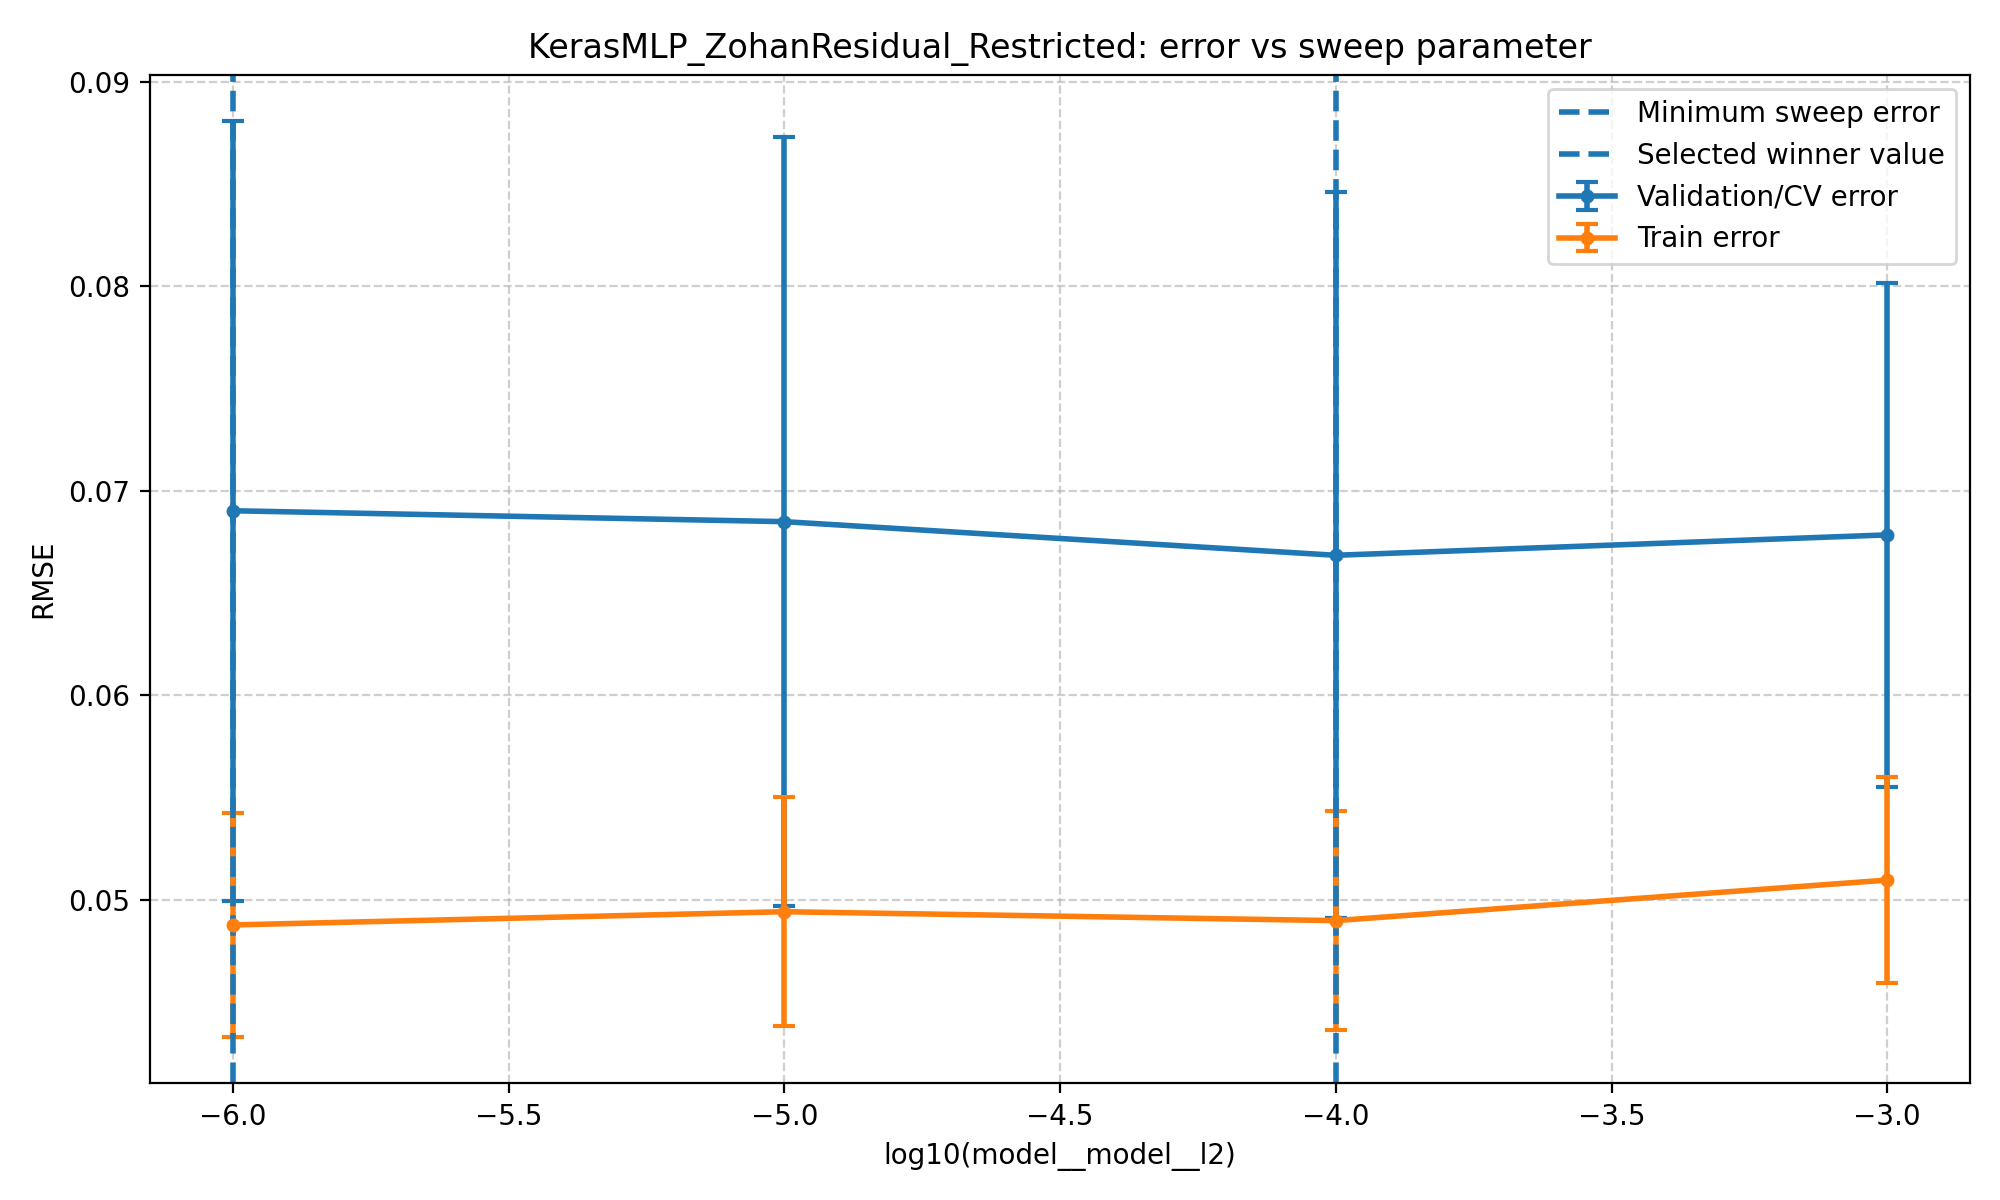
\includegraphics[width=0.82\textwidth]{Imagens/chap06/model_selection/sweep_l2_ZohanResidual.png}
\caption[Variação do erro com a regularização $L_2$ na arquitetura ZohanResidual]{Variação do erro de validação cruzada em função do hiperparâmetro de regularização $L_2$ para a arquitetura híbrida ZohanResidual. Como a estrutura do modelo é mantida fixa, a análise evidencia o efeito da regularização na capacidade de generalização, permitindo identificar a faixa de valores associada ao melhor desempenho preditivo. Fonte: Autor.}
\label{fig:error_sweepparam_best_model}
\end{figure}

Na Figura~\ref{fig:error_sweepparam_best_model}, observa-se que o erro de validação cruzada apresenta pequena variação entre os valores de regularização avaliados. Esse comportamento indica que, na etapa de ajuste restrito, a arquitetura híbrida ZohanResidual não dependeu fortemente de um valor específico de $\lambda_{L2}$ para manter bom desempenho preditivo. Em outras palavras, diferentemente de um cenário em que pequenas alterações no hiperparâmetro provocariam grandes oscilações no erro, o gráfico sugere um comportamento relativamente estável ao longo da faixa analisada.

O valor selecionado corresponde ao menor erro médio de validação cruzada entre as configurações avaliadas. No entanto, a proximidade entre os erros obtidos indica que o ganho associado a essa escolha pontual é limitado. Assim, a principal informação extraída da Figura~\ref{fig:error_sweepparam_best_model} não é apenas o valor ótimo de regularização, mas a baixa sensibilidade da arquitetura híbrida ao hiperparâmetro analisado. Essa estabilidade é relevante no contexto deste trabalho, pois reduz a dependência do desempenho em relação a uma configuração específica e reforça a robustez do modelo dentro da faixa operacional estudada.
\subsection{Comportamento do treinamento da rede neural de referência}

Antes da avaliação da arquitetura híbrida final, foi analisado o comportamento de treinamento da rede neural de referência, utilizada como base para a definição do procedimento de ajuste dos modelos neurais. Essa etapa permitiu verificar a evolução das perdas de treinamento e validação ao longo das épocas, bem como o funcionamento do critério de parada antecipada adotado no treinamento.

A Figura~\ref{fig:learning_curve_baseline} apresenta a evolução das perdas de treinamento e validação ao longo das épocas para a rede neural de referência. O ponto indicado pela linha tracejada corresponde à época selecionada automaticamente pelo mecanismo de \textit{EarlyStopping}.

\begin{figure}[H]
\centering
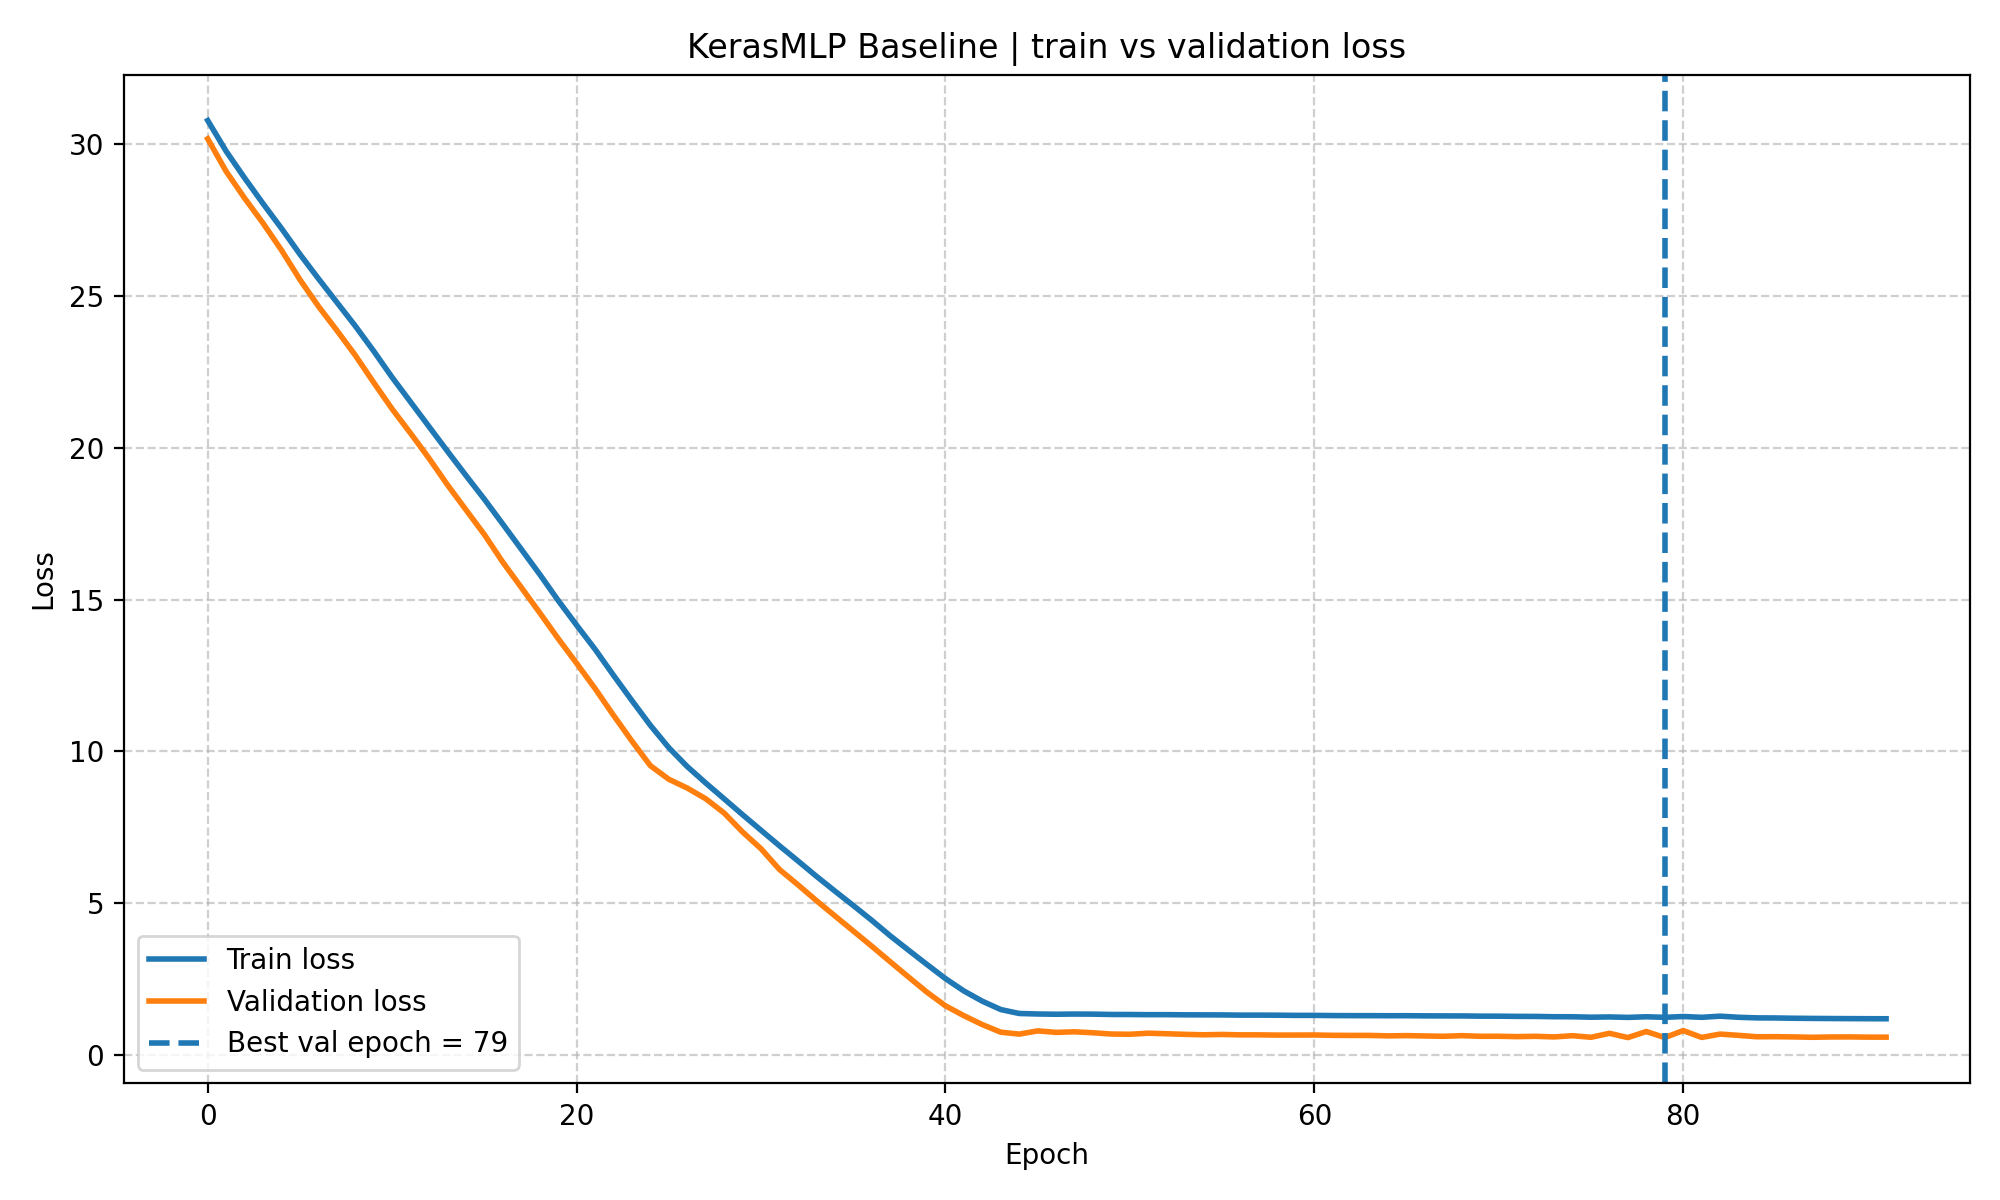
\includegraphics[width=0.78\textwidth]{Imagens/chap06/model_selection/learning_curve_baseline.png}
\caption[Curvas de treinamento e validação da rede neural de referência]{Curvas de erro para os conjuntos de treinamento e validação ao longo das épocas para a rede neural de referência. A linha tracejada indica a época selecionada pelo critério de parada antecipada (\textit{EarlyStopping}), utilizado para evitar sobreajuste e preservar a capacidade de generalização do modelo. Fonte: Autor.}
\label{fig:learning_curve_baseline}
\end{figure}

Observa-se que tanto a perda de treinamento quanto a perda de validação apresentam redução consistente ao longo das primeiras épocas, indicando aprendizado efetivo do modelo. A partir de aproximadamente 30 épocas, a melhoria na perda de validação torna-se marginal, levando ao acionamento do critério de \textit{EarlyStopping}, que interrompe o treinamento quando não são observadas melhorias adicionais relevantes na validação.

Esse mecanismo é particularmente importante em cenários com conjuntos de dados experimentais limitados, pois evita que a rede continue ajustando seus pesos após o ponto de melhor desempenho em validação. Dessa forma, reduz-se o risco de sobreajuste e aumenta-se a confiabilidade da comparação entre diferentes configurações de modelos neurais.

Com base nesse procedimento, a arquitetura híbrida ZohanResidual foi posteriormente avaliada como modelo final. Diferentemente da rede neural de referência, que aprende diretamente a relação entre as variáveis operacionais e as variáveis de saída, o modelo híbrido incorpora também informação proveniente do modelo físico reduzido. Assim, a rede passa a combinar a flexibilidade da modelagem orientada por dados com uma estimativa fenomenológica prévia do comportamento do sistema.

Dessa forma, a análise da rede de referência não representa o resultado final do trabalho, mas uma etapa necessária para estabelecer o procedimento de treinamento, seleção e controle de sobreajuste utilizado na avaliação das arquiteturas neurais. A partir dessa base, o modelo híbrido ZohanResidual foi selecionado por apresentar melhor desempenho preditivo, mantendo estabilidade de treinamento e boa capacidade de generalização dentro da faixa operacional estudada.
\subsection{Predições fora do conjunto de treinamento na validação cruzada}

A Figura 5.17 apresenta a comparação entre os valores experimentais e as predições obtidas para as amostras mantidas fora do treinamento em cada partição da validação cruzada. Essas predições, denominadas \textit{out-of-fold}, não correspondem a um conjunto de teste externo independente, mas permitem avaliar o desempenho do modelo em observações que não foram utilizadas no ajuste dos parâmetros durante a respectiva rodada de validação.

\begin{figure}[H]
\centering

\begin{subfigure}{0.32\textwidth}
\centering
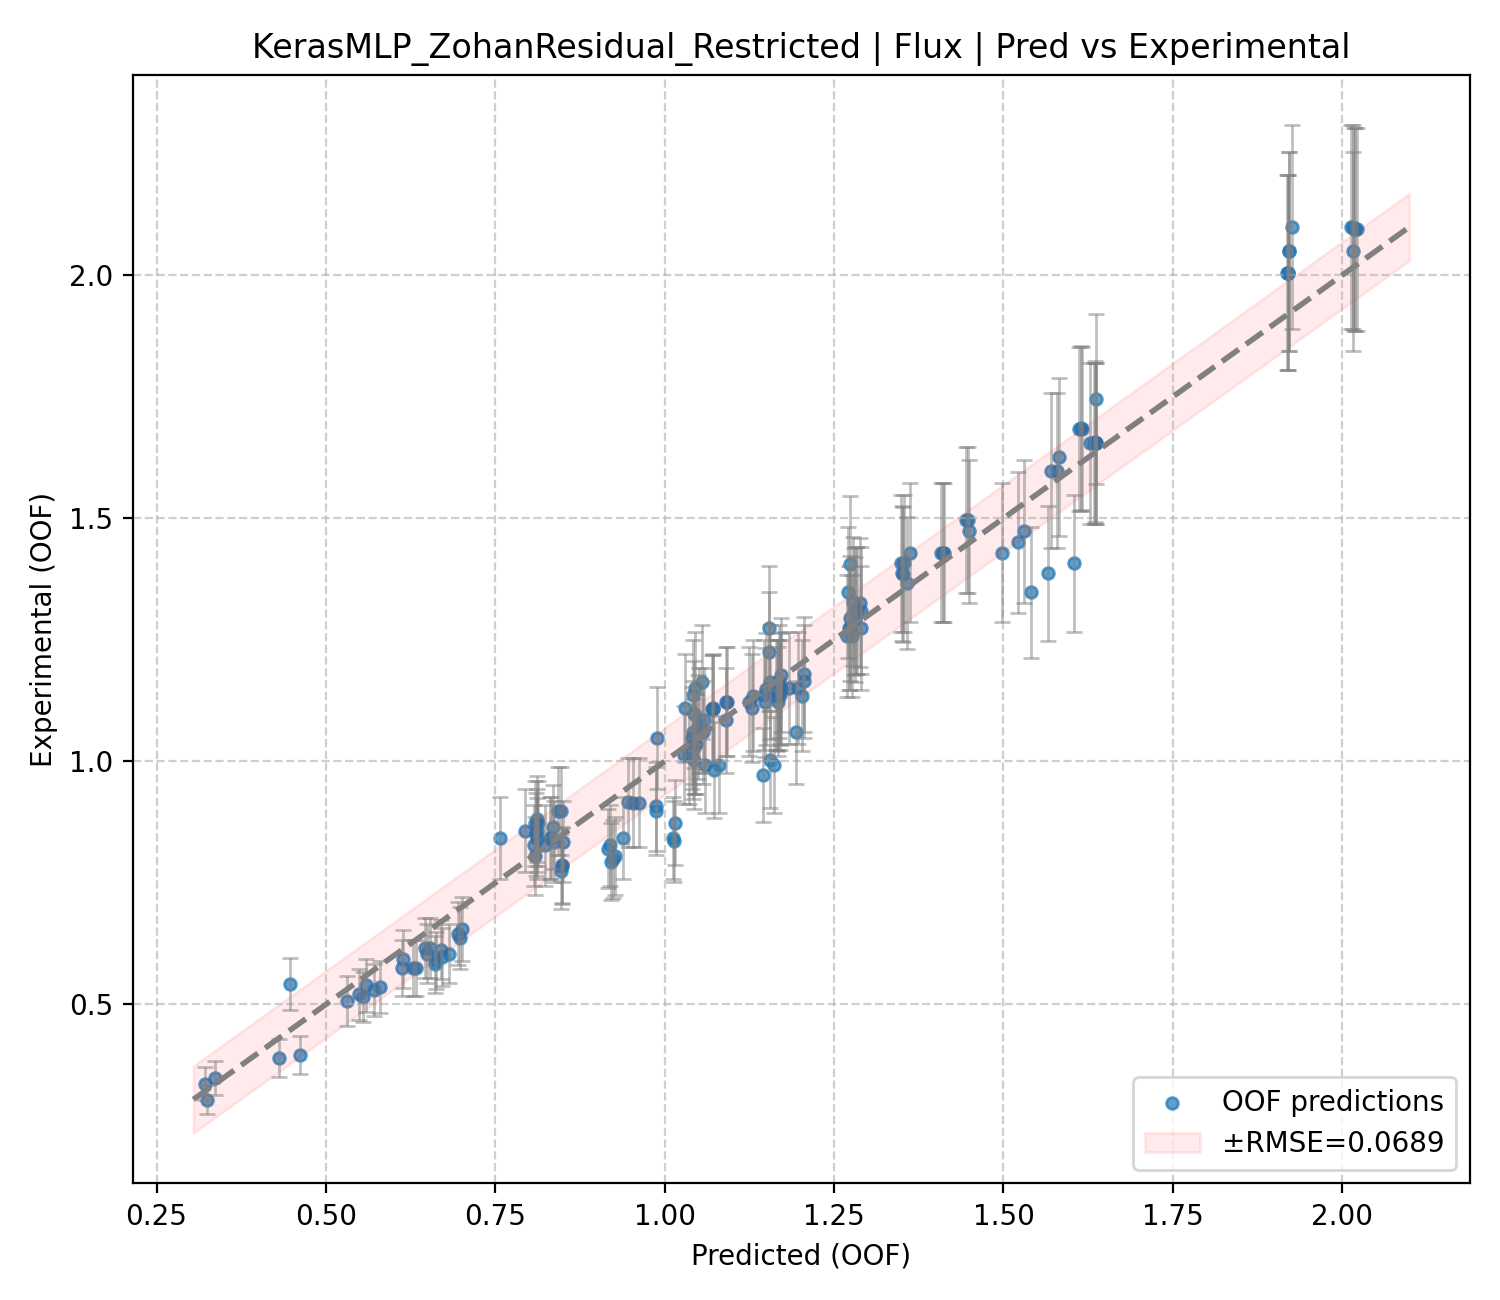
\includegraphics[width=\textwidth]{Imagens/chap06/model_selection/oof_KerasMLP_ZohanResidual_Restricted_Flux.png}
\caption{$Flux$}
\end{subfigure}
\hfill
\begin{subfigure}{0.32\textwidth}
\centering
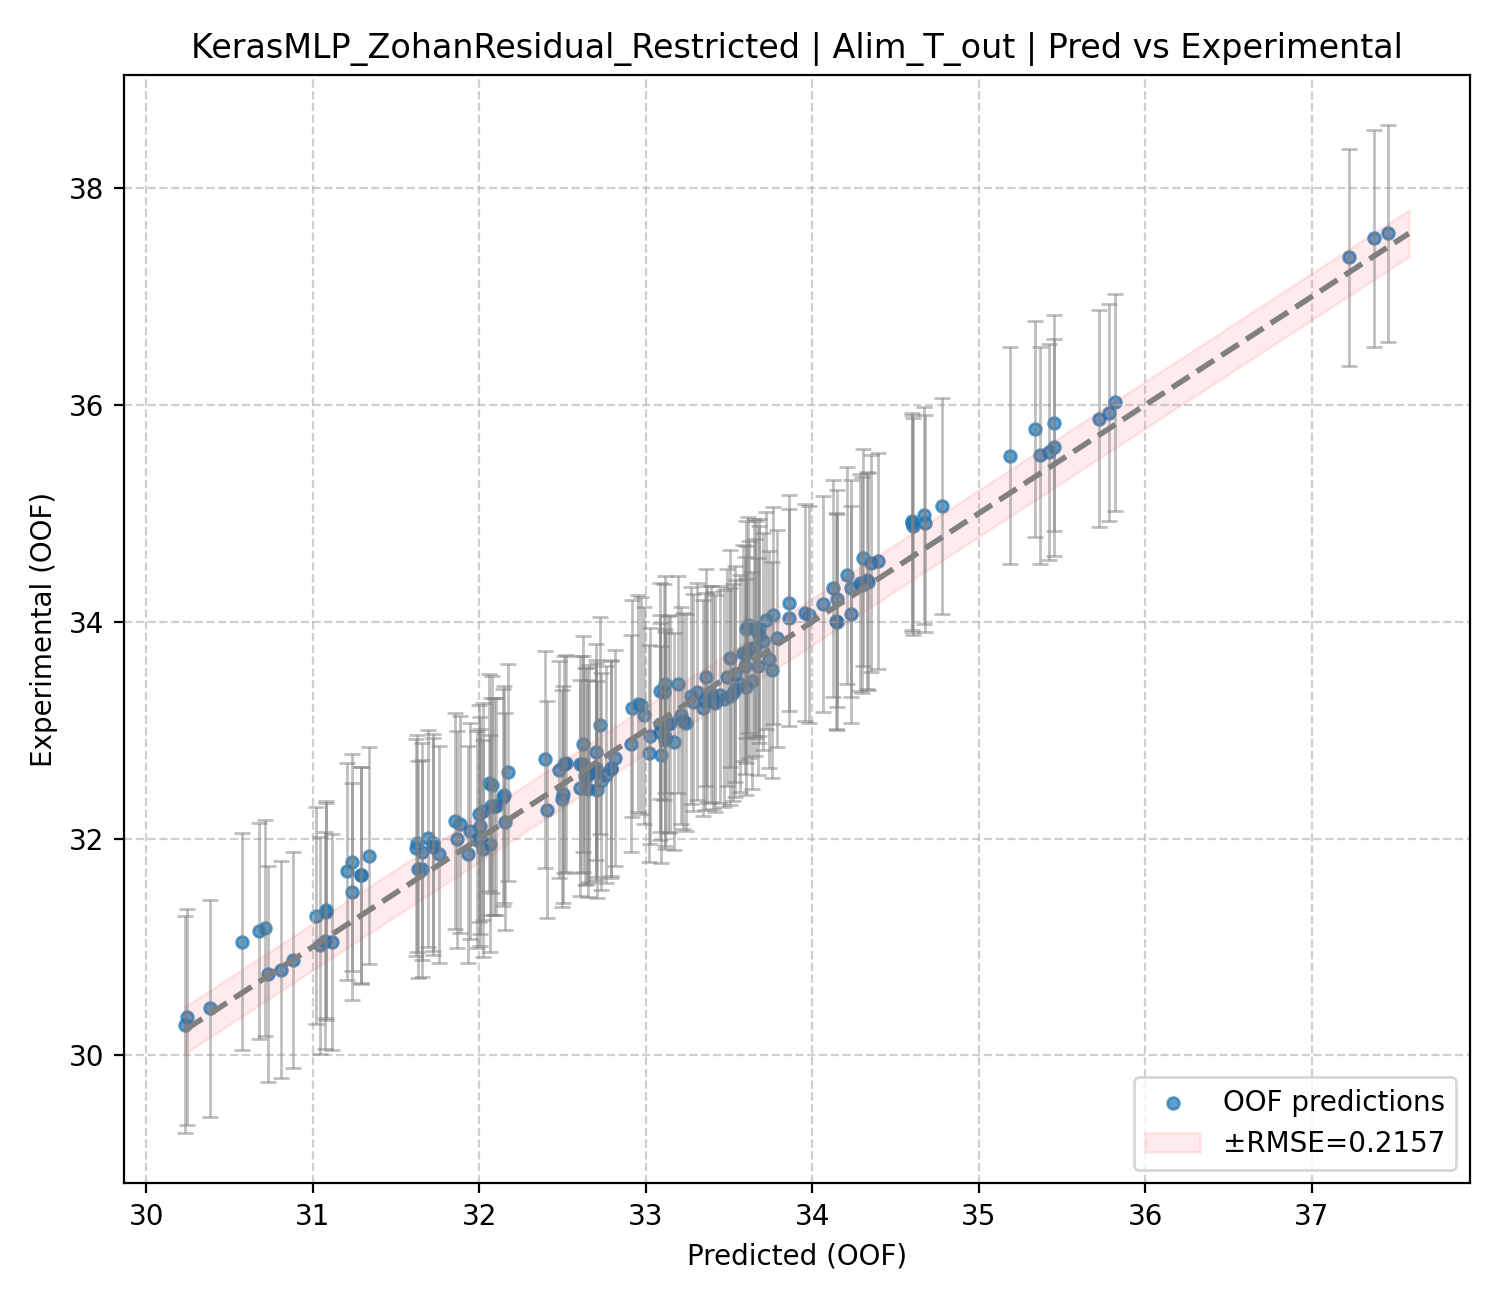
\includegraphics[width=\textwidth]{Imagens/chap06/model_selection/oof_KerasMLP_ZohanResidual_Restricted_Alim_T_out.png}
\caption{$Alim\_T_{out}$}
\end{subfigure}
\hfill
\begin{subfigure}{0.32\textwidth}
\centering
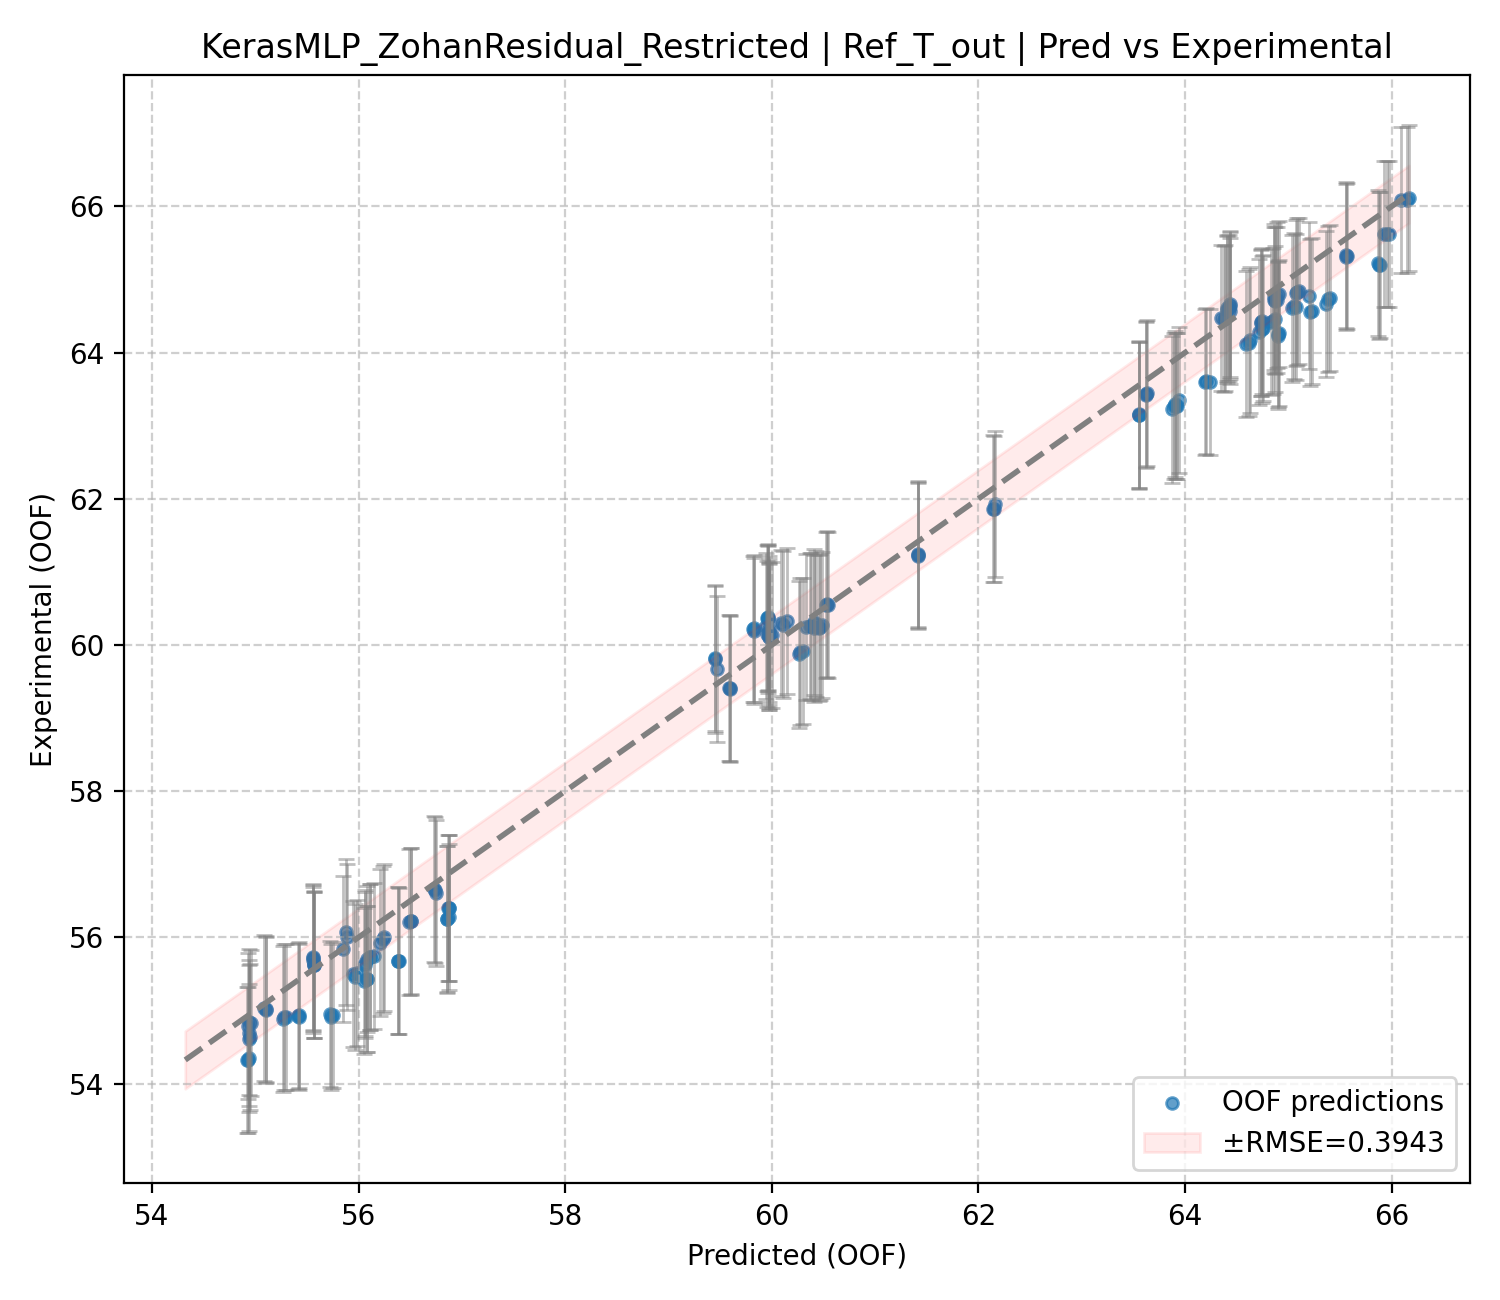
\includegraphics[width=\textwidth]{Imagens/chap06/model_selection/oof_KerasMLP_ZohanResidual_Restricted_Ref_T_out.png}
\caption{$Ref\_T_{out}$}
\end{subfigure}

\caption[Predições \textit{out-of-fold} do modelo ZohanResidual]{Predições \textit{out-of-fold} do modelo híbrido ZohanResidual para as três variáveis de saída do sistema. Os gráficos comparam os valores previstos e experimentais para o fluxo de permeado e as temperaturas de saída, considerando as amostras mantidas fora do treinamento em cada partição da validação cruzada. Fonte: Autor.}
\label{fig:best_model_oof_predictions}
\end{figure}

Observa-se concordância entre os valores experimentais e os valores previstos, especialmente para o alvo $Flux$, que foi priorizado no processo de seleção. A proximidade de grande parte dos pontos em relação à reta identidade indica que o modelo foi capaz de representar as principais tendências presentes nos dados experimentais. Ao mesmo tempo, as dispersões observadas em determinadas regiões do espaço de operação indicam que ainda existem desvios residuais, sobretudo em condições nas quais a variabilidade experimental ou a menor densidade de amostras pode dificultar a predição.

Em conjunto, os resultados apresentados ao longo desta análise indicam que a arquitetura híbrida selecionada combina bom desempenho preditivo com estabilidade de treinamento e baixa sensibilidade aos hiperparâmetros avaliados. Essas características são desejáveis em aplicações com conjuntos de dados experimentais, onde o risco de sobreajuste e a dependência do desempenho em relação à partição dos dados e às configurações escolhidas são fatores relevantes. Nesse sentido, a menor sensibilidade observada sugere maior robustez do modelo dentro da faixa operacional estudada.
\section{Comparação entre o modelo físico reduzido e o modelo final híbrido}
\label{subsec:comparacao_modelo_fisico_modelo_final}

Por fim, realizou-se a comparação entre o modelo físico reduzido utilizado como referência fenomenológica e o modelo final híbrido selecionado neste trabalho. Essa análise é central para a interpretação dos resultados, pois permite avaliar se a incorporação de técnicas de aprendizado de máquina, combinadas à informação física previamente disponível, trouxe ganhos efetivos em relação ao modelo físico 0D isolado.

O modelo físico reduzido representa uma descrição simplificada do processo V-AGMD, construída a partir de hipóteses fenomenológicas e relações de transferência de calor e massa. Embora esse tipo de abordagem seja fundamental para compreender o comportamento do sistema, sua capacidade preditiva pode ser limitada pelas simplificações adotadas e pela dificuldade de representar integralmente os efeitos acoplados presentes no processo. Nesse contexto, o modelo híbrido ZohanResidual foi avaliado como uma alternativa capaz de preservar a informação física fornecida pelo modelo 0D, ao mesmo tempo em que aprende, a partir dos dados experimentais, correções associadas ao comportamento real do sistema.

\begin{table}[H]
\centering
\caption{Comparação entre o modelo físico reduzido e o modelo híbrido final.}
\begin{tabular}{lccc}
\toprule
Modelo & RMSE$_{Alim}$ & RMSE$_{Ref}$ & RMSE$_{Flux}$ \\
\midrule
Modelo físico 0D & 1.613 & 0.927 & 0.215 \\
Modelo híbrido ZohanResidual & 0.290 & 0.385 & \textbf{0.061} \\
\bottomrule
\end{tabular}
\end{table}

\begin{figure}[H]
    \centering
    
    \begin{subfigure}[b]{0.48\linewidth}
        \centering
        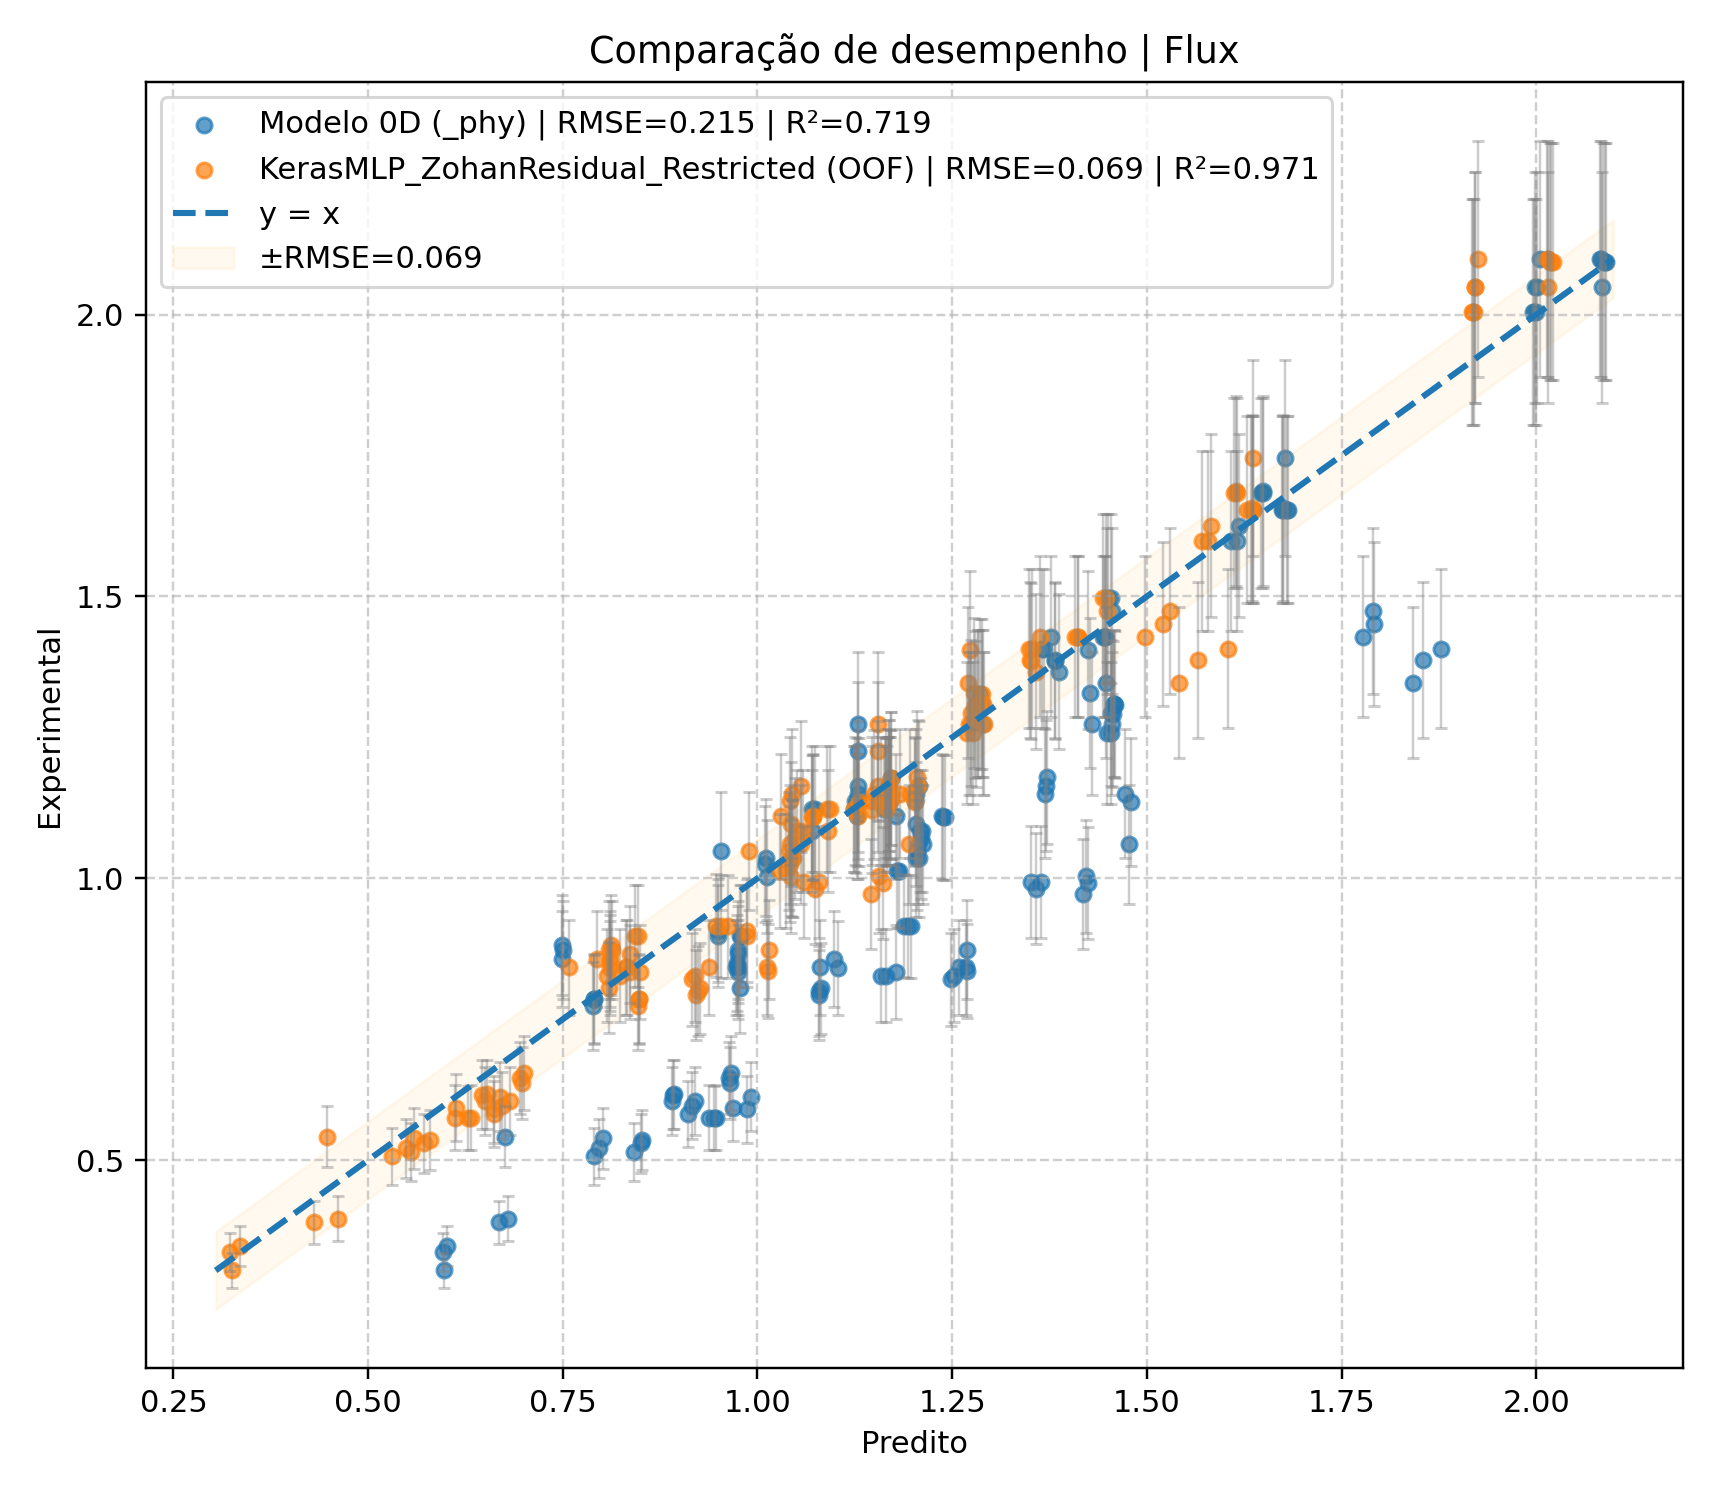
\includegraphics[width=\linewidth]{Imagens/chap06/overlay_ZohanResidual_Flux.png}
        \caption{Fluxo de permeado}
    \end{subfigure}
    \hfill
    \begin{subfigure}[b]{0.48\linewidth}
        \centering
        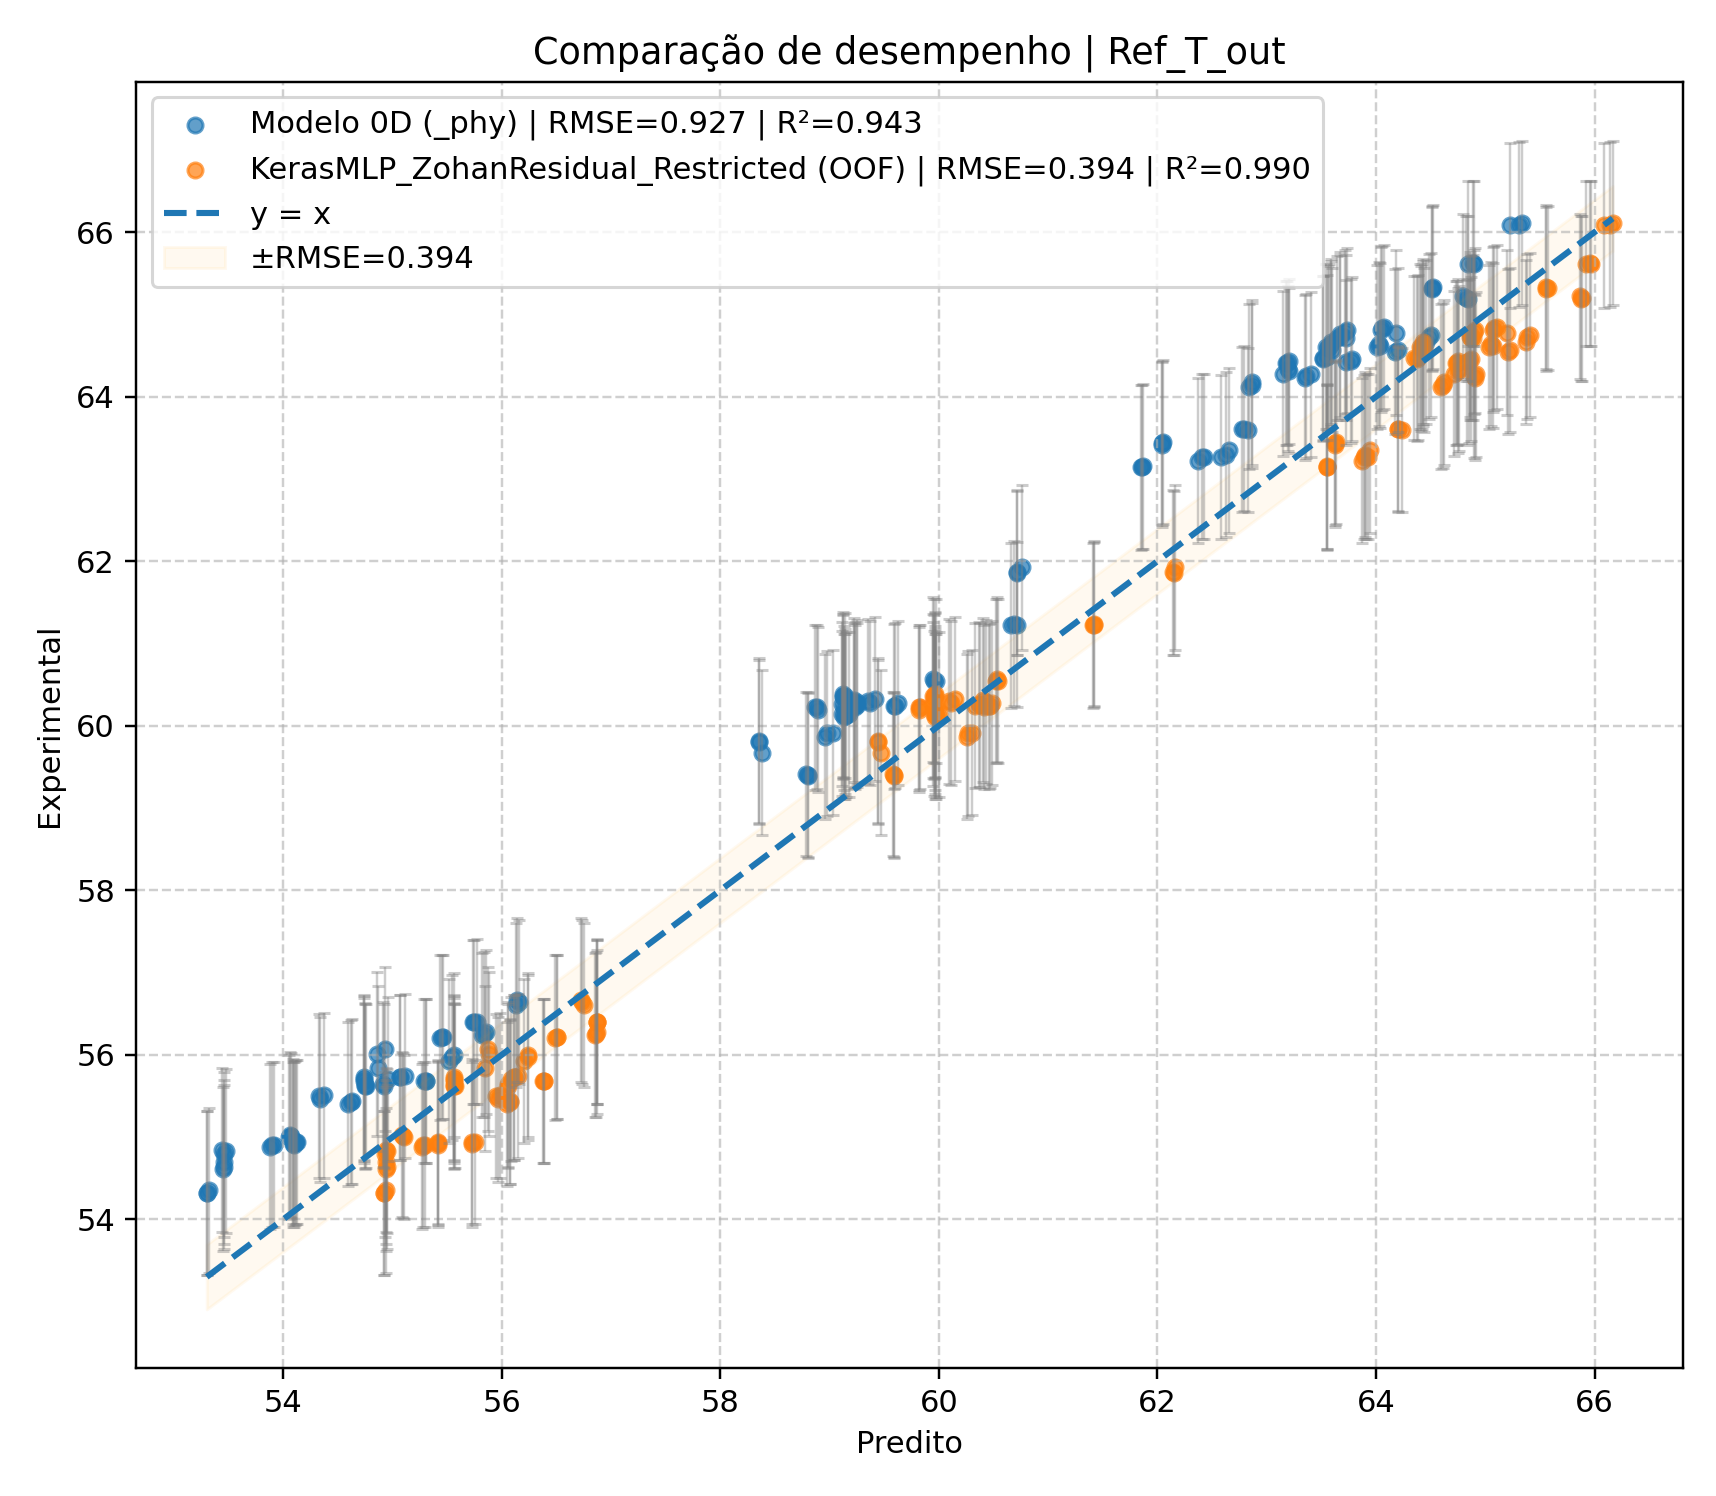
\includegraphics[width=\linewidth]{Imagens/chap06/overlay_ZohanResidual_Ref_T_out.png}
        \caption{Temperatura de saída do circuito de resfriamento}
    \end{subfigure}

    \vspace{0.5cm}

    \begin{subfigure}[b]{0.48\linewidth}
        \centering
        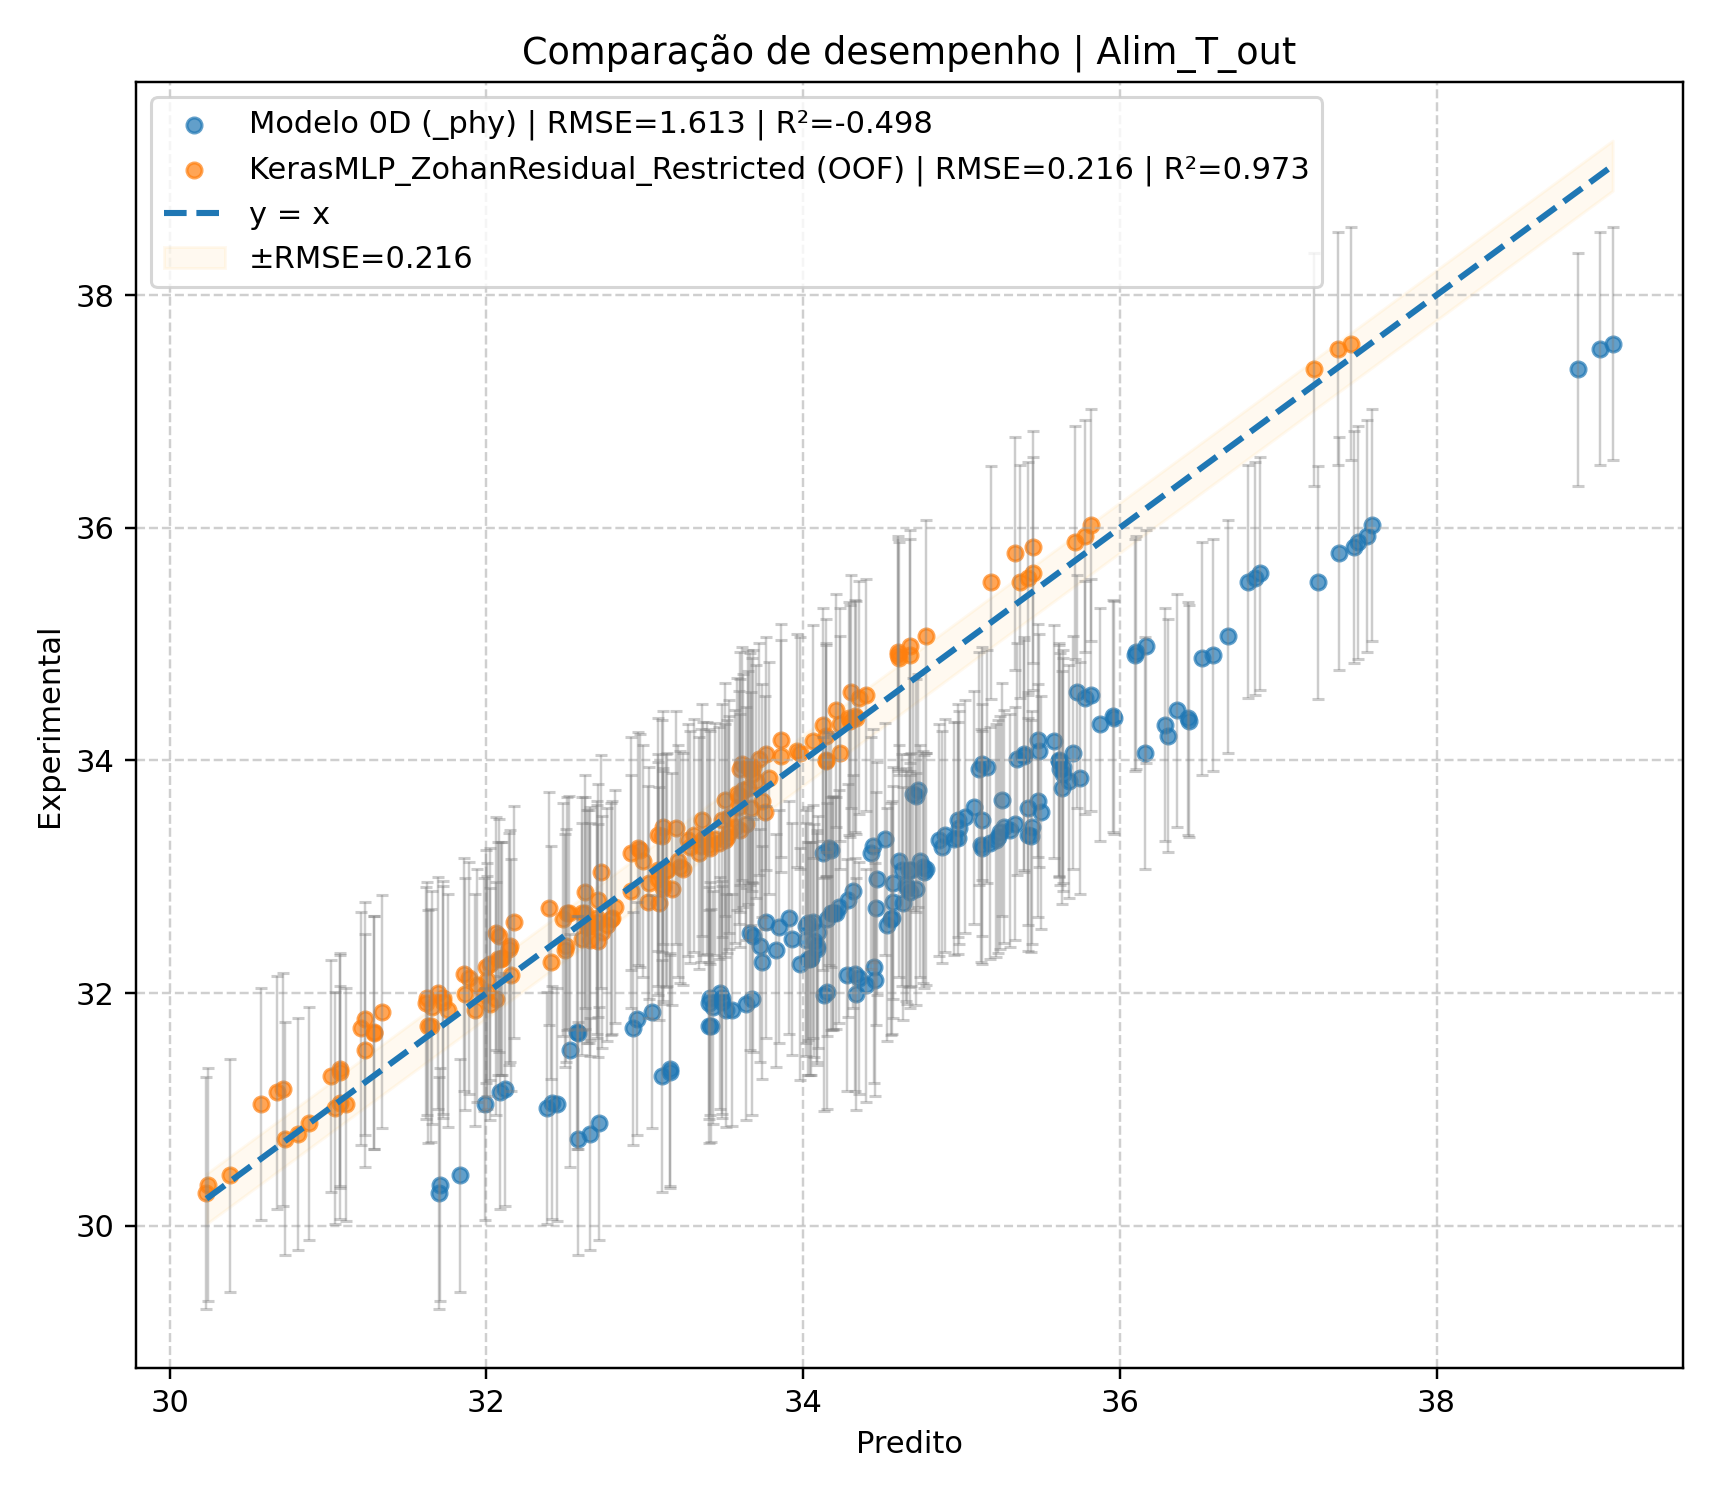
\includegraphics[width=\linewidth]{Imagens/chap06/overlay_ZohanResidual_Alim_T_out.png}
        \caption{Temperatura de saída da alimentação}
    \end{subfigure}

    \caption[Comparação entre valores experimentais e predições dos modelos físico e híbrido]{Comparação entre os valores experimentais e as predições do modelo físico 0D e do modelo híbrido ZohanResidual para as variáveis de saída do sistema. Os gráficos permitem avaliar a capacidade de cada abordagem em reproduzir o comportamento do fluxo de permeado e das temperaturas de saída ao longo dos dados experimentais, evidenciando o ganho preditivo obtido com a incorporação de informação orientada por dados. Fonte: Autor.}
    \label{fig:overlay_hibrido}
\end{figure}

Os resultados indicam que o modelo híbrido ZohanResidual apresentou redução expressiva do erro em relação ao modelo físico reduzido para as três variáveis analisadas. Para o fluxo de permeado, variável priorizada na seleção dos modelos, o RMSE foi reduzido de 0,215 para 0,061. Também foram observados ganhos nas temperaturas de saída, com redução do erro de 1,613 para 0,290 em $Alim\_T\_out$ e de 0,927 para 0,385 em $Ref\_T\_out$.

Esse resultado mostra que o modelo físico 0D, embora seja capaz de representar tendências gerais do sistema, não captura integralmente as relações presentes nos dados experimentais. A arquitetura híbrida, por sua vez, foi capaz de utilizar a informação física como referência inicial e aprender ajustes orientados pelos dados, reduzindo os desvios em relação às medições experimentais. Assim, o ganho obtido não decorre apenas do uso de uma rede neural mais flexível, mas da combinação entre uma representação fenomenológica do processo e uma etapa de correção empírica baseada nos dados disponíveis.

Dessa forma, a principal contribuição deste trabalho está em demonstrar que, para o sistema V-AGMD analisado, a abordagem híbrida apresentou vantagem em relação ao uso isolado do modelo físico reduzido. Esse resultado é particularmente relevante porque sistemas de destilação por membranas envolvem fenômenos acoplados de transferência de calor e massa, cuja modelagem puramente fenomenológica pode exigir hipóteses simplificadoras. A incorporação de aprendizado orientado por dados permite complementar essa descrição física, melhorando a capacidade preditiva dentro da faixa operacional estudada.

Portanto, a comparação entre o modelo físico 0D e o modelo híbrido ZohanResidual evidencia o valor da estratégia adotada ao longo deste trabalho: partir de uma base física conhecida, avaliar diferentes famílias de modelos e verificar se a informação experimental disponível poderia ser utilizada para melhorar a predição das variáveis de desempenho. Os resultados obtidos indicam que essa estratégia foi bem-sucedida, reforçando o potencial de abordagens híbridas físico-orientadas por dados como ferramenta de modelagem para sistemas V-AGMD.